\chapter[Self-supervised learning for brain cavity segmentation]{\onehalfspacing{Self-supervised learning for brain cavity segmentation simulating resections}}

\chaptermark{Self-supervised learning for brain cavity segmentation}  % short title for headers
\label{chap:resection}
\minitoc

\begin{center}
  \begin{minipage}[b]{0.9\linewidth}
    \small
    \textbf{Foreword\,}
    This chapter is adapted and contains content from the work presented in:
    \begin{itemize}
      \item \bibentry{perez-garcia_simulation_2020}
      \item \bibentry{perez-garcia_self-supervised_2021}
    \end{itemize}
  \end{minipage}
\end{center}

\doublespacing
\section{Introduction}

\subsection{Motivation}

Approximately one third of epilepsies are drug-resistant.
If the \ac{EZ}, i.e., ``the area of cortex indispensable for the generation of clinical seizures'' \cite{rosenow_presurgical_2001}, can be localized, resective surgery to remove the \ac{EZ} may be curative.
As previously mentioned, only 40\% to 70\% of patients with refractory focal epilepsy are seizure-free after surgery \cite{jobst_resective_2015}.
This is, in part, due to limitations identifying the \ac{EZ} during the presurgical evaluation.
Retrospective studies relating presurgical clinical features and resected brain structures to surgical outcome provide useful insights to guide \ac{EZ} resection \cite{jobst_resective_2015}.
To quantify resected structures, first, the \ac{RC} must be segmented on the postoperative \ac{MRI}.
A preoperative image with a corresponding brain parcellation can then be registered to the postoperative \ac{MRI} to identify resected structures.

\Ac{RC} segmentation is also necessary in other applications.
For neuro-oncology, the gross tumor volume, which is the sum of the \ac{RC} and residual tumor volumes, is estimated for postoperative radiotherapy \cite{ermis_fully_2020}.

Despite recent efforts to segment \acp{RC} in the context of brain cancer \cite{meier_automatic_2017,ermis_fully_2020}, little research has been published in the context of epilepsy surgery.
Furthermore, previous work is limited by the lack of benchmark datasets, released code or trained models, and evaluation is restricted to single-institution datasets used for both training and testing.


\subsection{Related works}

After surgery, \acp{RC} fill with \ac{CSF}.
This causes an inherent uncertainty in delineating \acp{RC} adjacent to structures such as sulci, ventricles or edemas.
Nonlinear registration has been presented to segment the \ac{RC} for epilepsy \cite{chitphakdithai_non-rigid_2010} and brain tumor \cite{chen_deformable_2015} surgeries by detecting non-corresponding regions between pre- and postoperative images.
However, evaluation of these methods was restricted to a very small number of images.
Furthermore, in cases with intensity changes due to the resection (e.g., brain shift, atrophy, fluid filling), non-corresponding voxels may not correspond to the \ac{RC}.

Decision forests were presented for brain cavity segmentation after glioblastoma surgery, using four \ac{MRI} modalities \cite{meier_automatic_2017}.
These methods, which aggregate hand-crafted features extracted from all  modalities to train a classifier, can be sensitive to signal inhomogeneity and unable to distinguish regions with intensity patterns similar to \ac{CSF} from \acp{RC}.
Recently, a 2D \ac{CNN} was trained to segment the \ac{RC} on \ac{MRI} slices in 30 glioblastoma patients \cite{ermis_fully_2020}.
They obtained a `median (interquartile range)' \ac{DSC} of 84 (10) compared to ground-truth labels by averaging predictions across anatomical axes to compute the 3D segmentation.
While these approaches require four modalities to segment the \ac{RC}, some of the modalities are often unavailable in clinical settings \cite{dorent_learning_2021}.
Furthermore, code and datasets are not publicly available, hindering a fair comparison across methods.
Applying these techniques requires curating a dataset with manually obtained annotations to train the models, which is expensive.

Unsupervised learning methods can leverage large, unlabeled medical image datasets during training.
In self-supervised learning, training instances are generated automatically from unlabeled data and used to train a model to perform a pretext task. %such as inpainting or image restoration.
The model can be fine-tuned on a smaller labeled dataset to perform a downstream task \cite{chen_self-supervised_2019}.
The pretext and downstream tasks may be the same.
For example, a \ac{CNN} was trained to reconstruct a skull bone flap by simulating craniectomies on CT scans \cite{matzkin_self-supervised_2020}.
Lesions simulated in chest CT of healthy subjects were used to train models for nodule detection, improving accuracy compared to training on a smaller dataset of real lesions \cite{pezeshk_seamless_2017}.

% Recovered from long version
Semi-supervised learning may be used when a large amount of unlabeled data is available.
A model trained on a labeled dataset (which may have been generated in a self-supervised setting) can generate pseudolabels for unlabeled data.
Uncertainty estimation may be used to select pseudolabeled instances with a low uncertainty for medical image segmentation tasks, improving model performance compared to using a random subset \cite{venturini_uncertainty_2020}.


\subsection{Contributions}

We present a self-supervised learning approach to train a 3D \ac{CNN} for brain \acp{RC} segmentation from \ac{T1w} \ac{MRI} without annotated data, by simulating resections during training.
We performed a comprehensive evaluation of our framework, assessing the effect of the resection simulation shape on performance and evaluating datasets from different institutions and pathologies.
We used uncertainty estimation as a selection criterion for pseudolabeled instances within our semi-supervised learning setting, which can be leveraged when postoperative \acp{MRI} without annotation are available, a typical scenario in clinical settings.

We ensure our work is reproducible by releasing the source code for resection simulation and \ac{CNN} training, the trained \ac{CNN}, and the evaluation dataset.
To the best of our knowledge, we introduce the first open annotated dataset of postoperative \ac{MRI} for epilepsy surgery.

\section{Methods}
\label{sec:methods}

\newcommand{\p}{\bm{p}}
\newcommand{\vv}{\bm{v}}
\newcommand{\X}{\bm{X}}
\newcommand{\Y}{\bm{Y}}
\newcommand{\M}{\bm{M}}
\newcommand{\U}{\bm{U}}
% \newcommand{\R}{\mathbb{R}}

\newcommand{\img}[2]{#1 : \Omega \to #2}
\newcommand{\binimg}[1]{\img{#1}{ \{ 0, 1 \} }}

\newcommand{\Dom}{\mathcal{D}}
\newcommand{\Tas}{\mathcal{T}}
\newcommand{\Xdo}{\mathcal{X}}
\newcommand{\Ydo}{\mathcal{Y}}
\newcommand{\fp}[1]{f_{\theta \text{#1}}}
\newcommand{\wt}{\widetilde}

% https://tex.stackexchange.com/a/466437/216202
\renewcommand*\st[1]{_{\textnormal{#1}}}

\newcommand{\post}{\st{postop}}
\newcommand{\pre}{\st{preop}}
\newcommand{\cav}{\st{cavity}}
\newcommand{\simul}{\st{sim}}
\newcommand{\lab}{\st{labeled}}
\newcommand{\unl}{\st{unlabeled}}


We describe our learning strategy in \cref{sec:learning_strategy} (\cref{fig:diagram_ijcars})
and introduce our \ac{RC} simulation in \cref{sec:simulation}.

\begin{figure}[ht]
  \centering
  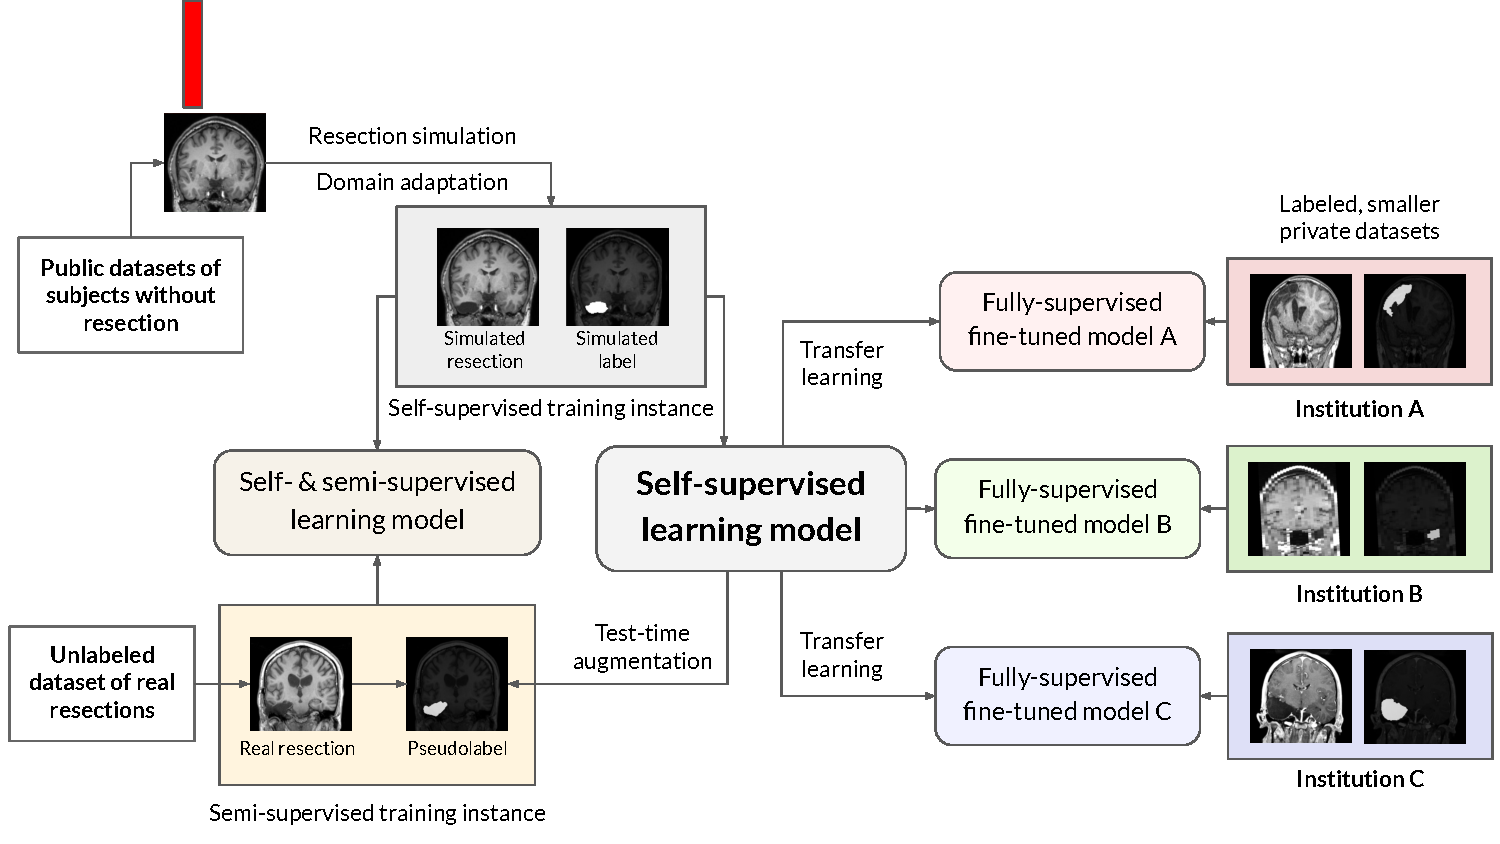
\includegraphics[trim={0 0 0 52},clip, width=\linewidth]{diagram_ijcars}
  \caption[Learning strategies for cavity segmentation]{
    Learning strategies.
    3D images without resections (top left) are modified by our resection simulation method to mimic postoperative images and their corresponding labels, generating training instances.
    These instances are used to train a baseline model in a self-supervised manner (middle).
    The baseline model generates pseudolabels from unlabeled images of patients who underwent resective surgery (bottom left).
    Instances from the \ac{RC} simulation and pseudolabeled dataset are used to train a new model in a self- and semi-supervised learning approach (left).
    The baseline model may be fine-tuned to improve its performance on small labeled datasets containing real resections from a single institution, using a standard fully-supervised learning approach (right).
  }
  \label{fig:diagram_ijcars}
\end{figure}

\subsection{Learning strategy}
\label{sec:learning_strategy}


\subsubsection{Problem statement}

\newcommand{\loss}{\mathcal{L}}
\newcommand{\expec}{\mathbb{E}}
\newcommand{\exppost}{\expec_{\Dom\post}}

The overall objective is to automatically segment resection cavities from postoperative \ac{T1w} \ac{MRI} using a \ac{CNN} $f_{\bm{\theta}}$ parameterized by weights $\bm{\theta}$.
Let $\X_{\text{post}} : \Omega \to \R$ and $\Y\cav  : \Omega \to \{ 0, 1 \}$ be a postoperative \ac{T1w} \ac{MRI} and its cavity segmentation label, respectively, where $\Omega \subset \R^3$.
$\X_{\text{post}}$ and $\Y_{\text{cavity}}$ are drawn from the data distribution $\Dom\post$.
In model training, the aim is to minimize the expected discrepancy between the label $\Y\cav$ and network prediction $f_{\bm{\theta}}(\X\post)$.
Let $\loss$ be a loss function that estimates this discrepancy (e.g., Dice loss).
The optimization problem for the network parameters $\bm{\theta}$ is:
\begin{equation}
  \bm{\theta}^* =
  \argmin_{\bm{\theta}}
  \exppost \left[
    \loss \left(
      f_{\bm{\theta}} \left( \X\post \right),
      \Y\cav
    \right)
  \right]
  \label{eq:problem_optimization}
\end{equation}


In a fully-supervised setting, a labeled dataset $D\post = \{ (\X_{\text{post}_i}, \Y_{\text{cavity}_i}) \}_{i = 1}^{n\post}$ is employed to estimate the expectation defined in \cref{eq:problem_optimization} as:
\begin{equation}
  \exppost \left[
    \loss \left(
      f_{\bm{\theta}} \left( \X\post \right), \Y\cav
    \right)
  \right]
  \approx \frac{1}{n\post} \sum_{i=1}^{n\post} \loss(f_{\bm{\theta}}(\X_{\text{post}_i}), \Y_{\text{post}_i})
  \label{eq:problem_optimization_fully}
\end{equation}

In practice, \acp{CNN} typically require an annotated dataset with a large $n\post$ to generalize well for unseen instances.
However, given the time and expertise required to annotate scans, $n\post$ is often small.
We present a method to artificially increase $n\post$ by simulating postoperative \acp{MRI} and associated labels from preoperative scans.


\subsubsection{Simulation for domain adaptation and self-supervised learning}
\label{sec:sim_res_self}

Let $D\pre = \{ \X_{\text{pre}_i} \}_{i = 1}^{n\pre}$ be a dataset of preoperative \ac{T1w} \ac{MRI}, drawn from the data distribution $\Dom\pre$.
We propose to generate a simulated postoperative dataset $D\simul = \{ (\X_{\text{sim}_i}, \Y_{\text{sim}_i}) \}_{i = 1}^{n\simul}$ using the preoperative dataset $D\pre$.
Specifically, we aim to build a generative model $\phi\simul : \X\pre \mapsto (\X\simul, \Y\simul)$ that transforms preoperative images into simulated, annotated postoperative images that imitate instances drawn from the postoperative data distribution $\Dom\post$.
$D\simul$ can then be used to estimate the expectation in \cref{eq:problem_optimization}:
\begin{equation}
  \exppost \left[\
    \loss\left(
      f_{\bm{\theta}} \left(\X\post \right), \Y\cav \right)
    \right]
    \approx \frac{1}{n\simul}\sum_{i=1}^{n\simul} \loss(f_{\bm{\theta}}(\X_{\text{sim}_i}),  \Y_{\text{sim}_i})
  \label{eq:problem_optimization_sim}
\end{equation}

Simulated images can be generated from any unlabeled preoperative dataset.
Therefore, the size of the simulated dataset can be much greater than the annotated dataset $D\post$, i.e., $n\simul\gg n\post$.
The network parameters $\bm{\theta}$ can be optimized by minimizing \cref{eq:problem_optimization_sim} using stochastic gradient descent, leading to a trained predictive function $f_{\bm{\theta_}{\text{sim}}}$.
Finally, $f_{\bm{\theta_}{\text{sim}}}$ can be fine-tuned on $D\post$ to improve performance on the postoperative domain $\Dom\post$.

\subsubsection{Leveraging unlabeled data from the target domain}
\label{sec:leveraging_semi}

Let $D\unl = \{ \X_{\text{postop}_i} \}_{i = 1}^{n\st{unl}}$ be a dataset comprising $n\st{unl}$ unlabeled postoperative images.
We propose to leverage $D\unl$ to build a better predictive model than using simulated resections only, employing a semi-supervised learning approach.
First, pseudolabels for each image $\X\post \in D\unl$ can be generated with $f_{\theta_{\text{sim}}}$ using data distillation, i.e., ensembling multiple predictions from transformed versions of $\X\post$.
Using the multiple predictions generated for pseudolabels, we estimate image-level segmentation uncertainty so that only instances with high reliability are used for training.
Finally, simulated resection instances and the selected pseudolabeled instances are used to train a new model $f_{\theta_{\text{sim+unl}}}$ in a hybrid self- and semi-supervised setting.


\paragraph{Generating pseudolabels using data distillation}

Data distillation is a method that ensembles predictions from multiple transformations applied to data, using a single model \cite{radosavovic_data_2017}.
We use Monte Carlo simulation to generate each pseudolabel with \ac{TTA}, which can improve the performance of segmentation models \cite{wang_aleatoric_2019}.
Let $n\st{u}$ represent the total number of simulation runs.
In the $i$-th simulation run,
the \ac{TTA} intensity and spatial transforms $T_\alpha$ and $T_\beta$ (\cref{sec:preprocessing_augmentation}) are applied to $\X\post$.
$\fp{sim}$ is used to predict $\wt{\Y}_{\theta\alpha\beta}'$, the probability of each voxel belonging to the cavity in the transformed space.
Finally, $T_\beta^{-1}$ is used to transform $\wt{\Y}_{\theta\alpha\beta}'$ back onto the space of $\X\post$:
\begin{equation}
    \wt{\Y}'_{\text{cavity}_i}
    = T_\beta^{-1}
    \circ \fp{sim}
    \circ T_\beta
    \circ T_\alpha
    \circ \X\post
    = T_\beta^{-1} \left( \wt{\Y}_{\theta\alpha\beta}' \right)
\end{equation}

We ensure that $T_\beta$ is invertible by using diffeomorphic spatial transformations.
To preserve image quality and ensure that probabilities stay within $[0, 1]$, we use tricubic and trilinear interpolation for $T_\beta$ and $T_\beta^{-1}$, respectively.

Predictions $P = \{ \wt{\Y}'_{\text{cavity}_i} \}_{i=1}^{n\st{u}}$ are averaged to obtain $\img{\wt{\Y}\cav}{[0, 1]}$, and the corresponding binary pseudolabel $\binimg{\widetilde{\Y}\cav}$ is obtained applying a threshold of 0.5 to $\wt{\Y}'\cav$.


\paragraph{Uncertainty estimation as selection criterion for pseudolabeled instances}

Images in $D\unl$ might have artifacts that limit the quality of the segmentation or include \acp{RC} not modeled by $\phi\simul$.
The corresponding noisy pseudolabels would hinder training of machine learning models.

As $n\st{unl}$ might be large, rather than performing manual quality control to select pseudolabels with high reliability for training, we use uncertainty estimation as an automated selection criterion \cite{venturini_uncertainty_2020}.

We use $n\st{unc}$ \ac{TTA} predictions to estimate aleatoric uncertainty, which captures noise inherent in the observation \cite{kendall_what_2017}.
Aleatoric uncertainty can indicate segmentation quality and is a successful selection criterion of pseudolabels in semi-supervised learning settings for medical image segmentation \cite{wang_aleatoric_2019,venturini_uncertainty_2020}.

Let $L = \{ l_i \}_{i = 1}^{n\st{unc}}$ denote the set of (soft) volumes of the segmented cavity for each prediction, where $l_i$ is the sum of all probabilities in the $i$-th prediction $\wt{\Y}'_{\text{cavity}_i} \in P$.
We use the \ac{CQV} of the volumes \cite{zwillinger_crc_1999,wang_aleatoric_2019} to estimate the image-level uncertainty $u : L \to \left[0, 1\right]$:
\begin{equation}
    u = \frac{q_3 - q_1}{q_3 + q_1}
\end{equation}
where $q_1$ and $q_3$ are the first and third quartiles of $L$, respectively.
The \ac{CQV} is agnostic to the volume of the segmented \ac{RC} and therefore avoids bias introduced by naturally-occurring uncertainty along the resection boundaries \cite{jungo_analyzing_2020}.
Finally, training instances with an associated prediction uncertainty $u(f_{\theta\alpha\beta}, \X\post, n\st{unc})$ below a threshold $t\st{unc}$ are combined with self-labeled instances (\cref{sec:sim_res_self}) to train a new model.

\subsection{Resection simulation for self-supervised learning}
\label{sec:simulation}

\newcommand{\AAA}{\bm{A}}
\newcommand{\NN}{\mathcal{N}}


$\phi\simul$ takes images from $\Dom\pre$ to generate training instances by simulating a realistic shape, location and intensity pattern for the \ac{RC}.
We present simulation of cavity shape and label in \cref{sec:cavity,sec:cavity_constrain}, respectively.
In \cref{sec:texture_cavity}, we present our method to generate the resected image.


\subsubsection{Initial cavity shape}
\label{sec:cavity}

To simulate a realistic \ac{RC}, we consider its topological and geometric properties: it is a single volume with a non-smooth boundary.
We generate a geodesic polyhedron with frequency $f$ by subdividing the edges of an icosahedron $f$ times and projecting each vertex onto a parametric sphere with a unit radius centered at the origin.
This polyhedron models a spherical surface $S = \{ V, F \}$ with vertices
$
  V = \left\{
    \vv_i \in \R^3
  \right\}
  _{i = 1}^{n_V}
$
and faces
$
  F = \left\{
    \bm{f}_k \in \mathbb{N}^3
  \right\}
  _{k = 1}^{n_F}
$, where $n_V$ and $n_F$ are the number of vertices and faces, respectively.
%
Each face $\bm{f}_k = \{ i_1^k, i_2^k, i_3^k \}$ is a sequence of three non-repeated vertex indices.

To create a non-smooth surface, $S$ is perturbed with simplex noise \cite{perlin_improving_2002}, a procedural noise generated by interpolating pseudorandom gradients on a multidimensional simplicial grid.
We chose simplex noise as it simulates natural-looking textures or terrains and is computationally efficient for multiple dimensions.
The noise $\eta : \R^3 \to [-1, 1]$ at point $\p \in \R^3$ is a weighted sum of the noise contribution for $\omega$ different octaves, with weights $\{\gamma ^ {n - 1}\}_{n = 1}^{\omega}$ controlled by the persistence parameter $\gamma$.
The displacement $\delta$ of a vertex $\vv$ is:
\begin{equation}
  \delta(\vv)
  = \eta \left( \frac{\vv + \bm{\mu} }{\zeta}, \omega, \gamma \right)
\end{equation}
where
$\zeta$ is a scaling parameter to control smoothness
and $\bm{\mu}$ is a shifting parameter that adds stochasticity
(equivalent to a random number generator seed).
%
Each vertex $\vv_i$ is displaced radially to create a perturbed sphere:
$
V_{\delta}
  = \left\{
  \vv_i
  + \delta(\vv_i)
  \frac{\vv_i}{\|\vv_i\|}
  \right\}
  _{i = 1}^{n_V}
  = \left\{
  \vv_{\delta i}
  \right\}
  _{i = 1}^{n_V}
$.

Next, a series of transforms is applied to $V_{\delta}$ to modify the mesh's volume and shape.
To add stochasticity, random rotations around each axis are applied to $V_{\delta}$ with the rotation transform
$T\st{R}(\bm{\theta}\st{r}) = R_x(\theta_x) \circ R_y(\theta_y) \circ R_z(\theta_z)$,
where~$\circ$~indicates a transform composition and
$R_i(\theta_i)$ is a rotation of $\theta_i$ radians around axis $i$.
$T\st{S}(\bm{r})$ is a scaling transform,
where $(r_1, r_2, r_3) = \bm{r}$ are semiaxes of an ellipsoid
with volume $v$ used to model the cavity shape.
The semiaxes are computed as
$r_1 = r$, $r_2 = \lambda r$ and $r_3 = r /\lambda$,
where $r = (3 v / 4)^{1/3}$ and
$\lambda$ controls the semiaxes length ratios\footnote{
  Note the volume of an ellipsoid with semiaxes $(a, b, c)$ is $v = \frac{4}{3} \pi a b c$.
}.
These transforms are applied to $V_{\delta}$ to define the initial \ac{RC} surface $S\st{E} = \{ V\st{E}, F \}$, where
$V\st{E} =
\{
  T\st{S}(\bm{r})
  \circ T\st{R}(\bm{\theta}\st{r})(
    \vv_{\delta i})
\}
_{i = 1}^{n_V}
$.


\subsubsection{Cavity label}
\label{sec:cavity_constrain}


\begin{figure}
  \centering
  % \captionsetup[subfigure]{justification=centering}
  \begin{subfigure}{0.3\textwidth}
    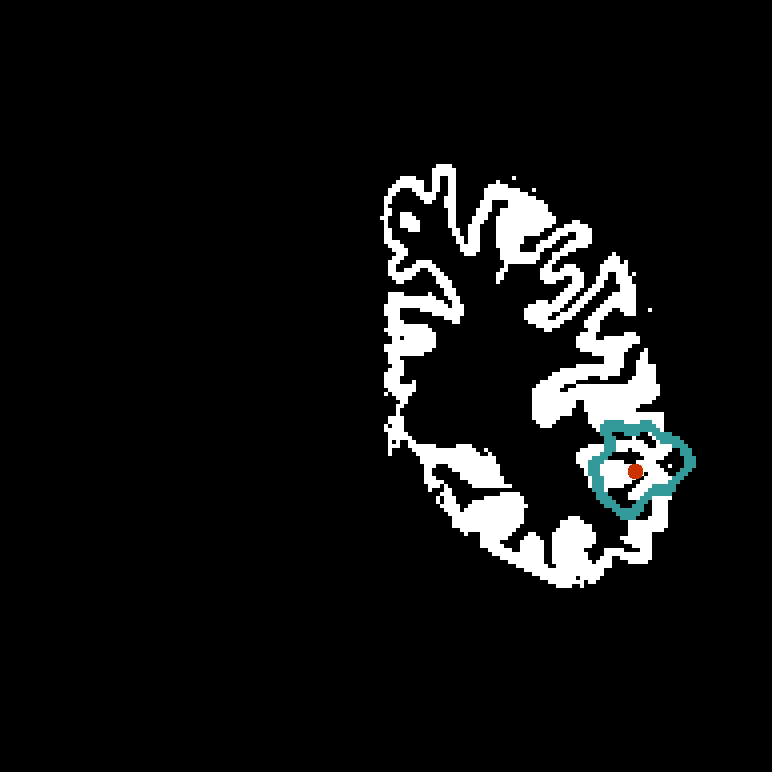
\includegraphics[width=0.8\linewidth]{Ma}
    \caption{$S_a$ on $\M\st{GM}^h$\label{fig:sama}}
  \end{subfigure}
  \begin{subfigure}{0.3\textwidth}
    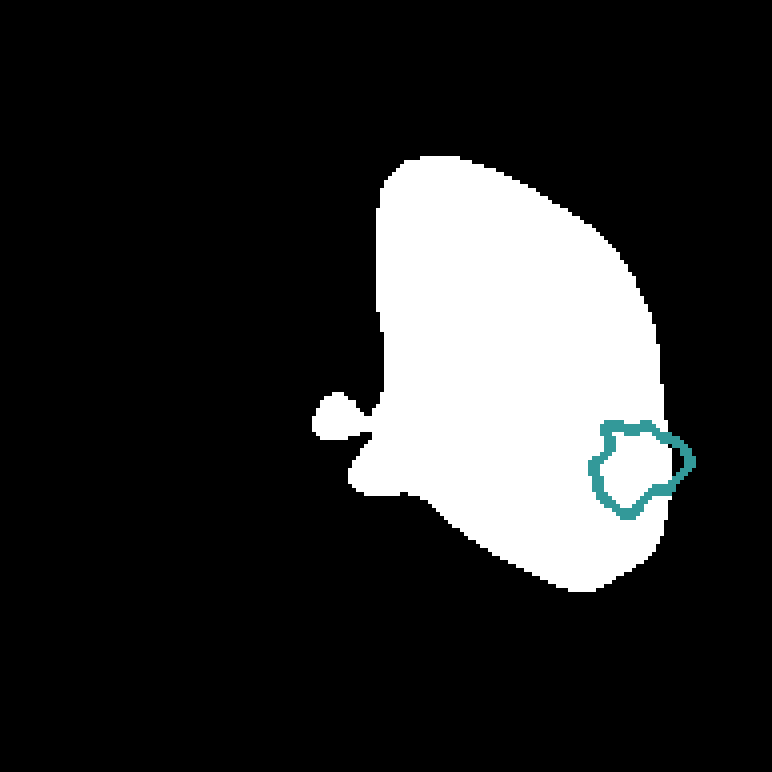
\includegraphics[width=0.8\linewidth]{Mb}
    \caption{$S_a$ on $\M\st{R}^h$\label{fig:samb}}
  \end{subfigure}
  \begin{subfigure}{0.3\textwidth}
    
\includegraphics[width=0.8\linewidth]{Mr}
    \caption{$\Y\simul = \M_{S_a} \odot \M\st{R}^h$\label{fig:mr}}
  \end{subfigure}

  \caption[Simulation of the ground-truth cavity label]{
    Simulation of the ground-truth cavity label.
    $S_a$ (blue) is computed by centering $S\st{E}$ on $\bm{a}$, a random positive voxel (red) of $\M\st{GM}^h$ (\subref{fig:sama}).
    $\M_{S_a}$ is a binary mask derived from $S_a$.
    $\Y\simul$ (\subref{fig:mr}) is the intersection of $\M_{S_a}$ and $\M\st{R}^h$ (\subref{fig:samb}).
  }
  \label{fig:shape}
\end{figure}



The simulated \ac{RC} should not span both hemispheres or include extracerebral tissues such as bone or scalp.
This section describes our method to ensure that the \ac{RC} appears in anatomically plausible regions.

A \ac{T1w} \ac{MRI} is defined as $\X\pre : \Omega \to \R$.
A full brain parcellation $\bm{P} : \Omega \to Z$ is generated \cite{cardoso_geodesic_2015} for $\X\pre$,
where $Z$ is the set of segmented structures.
A cortical gray matter mask $\M\st{GM}^h : \Omega \to \{0, 1\}$
of hemisphere $h$ is extracted from $\bm{P}$,
where $h$ is randomly chosen from $H = \{\text{left}, \text{right}\}$ with equal probability.

A ``resectable hemisphere mask'' $\M\st{R}^h$ is generated from $\bm{P}$ and $h$ such that $\M\st{R}^h (\p) = 1$ if
${\bm{P}(\p) \neq \{M\st{BG}, M\st{BT}, M\st{CB}, M_{\hat{h}} \} }$
and $0$ otherwise,
where $M\st{BG}$, $M\st{BT}$, $M\st{CB}$ and $M_{\hat{h}}$ are the labels in $Z$ corresponding to the background, brainstem, cerebellum and contralateral hemisphere, respectively.
$\M\st{R}^h$ is smoothed using a series of binary morphological operations, for realism.


A random voxel $\bm{a} \in \Omega$ is selected such that $\M\st{GM}^h(\bm{a}) = 1$.
A translation transform $T\st{T}(\bm{a} - \bm{c})$ is applied to $S\st{E}$ so $S_a = T\st{T}(\bm{a} - \bm{c}) (S\st{E})$ is centered on $\bm{a}$.

A binary image $\binimg{\M_{S_a}}$ is generated from $S_a$ such that $\M_{S_a}(\p) = 1$ for all $\p$ within $S_a$ and $\M_{S_a}(\p) = 0$ outside.
Finally, $\M_{S_a}$ is restricted by $\M\st{R}^h$ to generate the cavity label $\Y\simul = \M_{S_a} \odot \M\st{R}^h$, where $\odot$ represents the Hadamard product.
\cref{fig:shape} illustrates the process.



\subsubsection{Simulating cavities filled with CSF}
\label{sec:texture_cavity}

Brain \acp{RC} are typically filled with \ac{CSF}.
To generate a realistic \acs{CSF} texture,
we create a ventricle mask
${\M\st{V} : \Omega \to \{ 0, 1 \}}$ from $\bm{P}$, such that
$\M\st{V}(\p) = 1$ for all $\p$ within the ventricles and
$\M\st{V}(\p) = 0$ outside.
Intensity values within the ventricles are assumed to have
a normal distribution \cite{gudbjartsson_rician_1995}
with a mean $\mu\st{CSF}$ and standard deviation $\sigma\st{CSF}$
calculated from voxel intensity values in
$\{ \X\pre(\p) \mid \p \in \Omega \land \M\st{V}(\p) = 1 \}$.
A \acs{CSF}-like image is then generated as $\X\st{CSF}(\p) \sim \NN (\mu\st{CSF}, \sigma\st{CSF}), \forall \p \in \Omega$.


We use $\Y\simul$ to guide blending of $\X\st{CSF}$ and $\X\pre$ as follows.
A Gaussian filter is applied to $\Y\simul$ to obtain a smooth alpha channel $\img{\AAA_\alpha}{[0, 1]}$ defined as
$
  \AAA_\alpha
  = \Y\simul
  * \bm{G}_{\NN}(\bm{\sigma}),
$
where
$*$ is the convolution operator
and $\bm{G}_{\NN}(\bm{\sigma})$ is a 3D Gaussian kernel with standard deviations
$\bm{\sigma} = (\sigma_x, \sigma_y, \sigma_z)$.
Then, $\X\st{CSF}$ and $\X\pre$ are blended by the convex combination
\begin{equation}
  \X\simul
  = \AAA_\alpha \odot \X\st{CSF}
  + (1 - \AAA_\alpha) \odot \X\pre
\end{equation}

We use $\bm{\sigma} > 0$ to mimic partial-volume effects at the cavity boundary.
The blending process is illustrated in \cref{fig:texture}.


\begin{figure}
  \centering
  \captionsetup[subfigure]{aboveskip=3pt, belowskip=5pt}

  \begin{subfigure}{0.15\textwidth}
    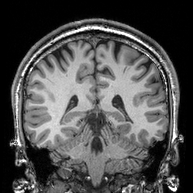
\includegraphics[width=0.99\linewidth]{texture_mri}
    \caption{\label{fig:tmri}}
  \end{subfigure}
  \begin{subfigure}{0.15\textwidth}
    
\includegraphics[width=0.99\linewidth]{texture_checkerboard}
    \caption{\label{fig:checkerboard}}
  \end{subfigure}
  \begin{subfigure}{0.15\textwidth}
    
\includegraphics[width=0.99\linewidth]{Mr}
    \caption{\label{fig:tmh}}
  \end{subfigure}
  \begin{subfigure}{0.15\textwidth}
    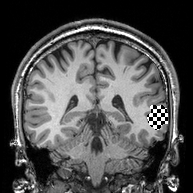
\includegraphics[width=0.99\linewidth]{texture_hard}
    \caption{\label{fig:blh}}
  \end{subfigure}
  \begin{subfigure}{0.15\textwidth}
    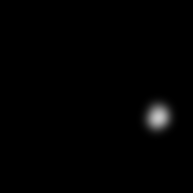
\includegraphics[width=0.99\linewidth]{texture_mask_soft}
    \caption{\label{fig:tms}}
  \end{subfigure}
  \begin{subfigure}{0.15\textwidth}
    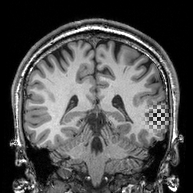
\includegraphics[width=0.99\linewidth]{texture_soft}
    \caption{\label{fig:bls}}
  \end{subfigure}

  \caption[Simulation of resected image using alpha blending]{
    Simulation of resected image $\X\simul$.
    We use a checkerboard for visualization.
    Two scalar-valued images $\X\pre$ (\subref{fig:tmri})
    and $\X_2$ (\subref{fig:checkerboard})
    are blended using $\Y\simul$ (\subref{fig:tmh})
    and $\sigma_i = \SI{0}{\milli \meter}$ to create an image with hard boundaries (\subref{fig:blh})
    and $\sigma_i = \SI{5}{\milli \meter}$ (\subref{fig:tms})
    for an image with soft boundaries (\subref{fig:bls}),
    mimicking partial-volume effects.
  }
  \label{fig:texture}
\end{figure}


\section{Experiments and results}
\label{sec:experiments_and_results}

\subsection{Data}
\label{sec:data}

\cref{tab:data} summarizes the datasets used for evaluation.


\newcommand{\zoom}[3]{$ #1 \times #2 \times #3 $}
\newcommand{\mr}[2]{\multirow{#1}{*}{#2}}
\newcommand{\mrsp}[4]{\mr{#1}{\zoom{#2}{#3}{#4}}}

\begin{table}
  \small
  \centering
  \caption[Datasets summary]{
    Datasets used in this study.
    Where multiple resolutions are present, the minimum, mean and maximum for each dimension are shown.
    `\acs{T1wCE}' indicates that gadolinium was administered for contrast enhancement.
  }
  \label{tab:data}
  \begin{tabular}{lclccc}
    \toprule
    \textbf{Dataset} & \textbf{Modality} & \textbf{Resolution (mm)} & \textbf{Subjects} & \textbf{Surgery} & \textbf{Annotated} \\
    \midrule
    \mr{3}{\textbf{IXI}}     &          \mr{3}{\ac{T1w}} & \zoom{0.94}{0.94}{1.20}  &       \mr{3}{566} &          \mr{3}{-} &          \mr{3}{-} \\
                             &                           & \zoom{0.94}{0.94}{1.20}  &                   &                    &                    \\
                             &                           & \zoom{0.98}{0.98}{1.20}  &                   &                    &                    \\
    \midrule
    \textbf{ADNI}            &                  \ac{T1w} & \zoom{1.00}{1.00}{1.00}  &               467 &                  - &                  - \\
    \midrule
    \mr{3}{\textbf{OASIS}}   &          \mr{3}{\ac{T1w}} & \zoom{1.00}{1.00}{1.00}  &       \mr{3}{780} &          \mr{3}{-} &          \mr{3}{-} \\
                             &                           & \zoom{1.05}{1.01}{1.02}  &                   &                    &                    \\
                             &                           & \zoom{1.20}{1.05}{3.00}  &                   &                    &                    \\
    \midrule
    \mr{3}{\textbf{EPISURG}} &          \mr{3}{\ac{T1w}} & \zoom{0.75}{0.75}{0.75}  &       \mr{3}{430} &   \mr{3}{Epilepsy} &        \mr{3}{133} \\
                             &                           & \zoom{0.96}{0.96}{1.08}  &                   &                    &                    \\
                             &                           & \zoom{1.09}{1.09}{1.60}  &                   &                    &                    \\
    \midrule
    \textbf{Milan}           &                  \ac{T1w} & \zoom{0.46}{0.46}{0.90}  &                20 &           Epilepsy &                 20 \\
    \midrule
    \mr{3}{\textbf{Strasbourg}} & \mr{3}{\ac{T1w} \& \acs{T1wCE}} & \zoom{0.23}{0.23}{0.50}  &        \mr{3}{33} &   \mr{3}{Epilepsy} &         \mr{3}{33} \\
                             &                           & \zoom{0.61}{0.61}{2.79}  &                   &                    &                    \\
                             &                           & \zoom{1.00}{1.00}{5.00}  &                   &                    &                    \\
    \midrule
    \mr{3}{\textbf{Paris}}   &          \mr{3}{\ac{T1w}} & \zoom{0.47}{0.47}{0.49}  &        \mr{3}{19} &   \mr{3}{Epilepsy} &         \mr{3}{19} \\
                             &                           & \zoom{0.82}{0.76}{1.06}  &                   &                    &                    \\
                             &                           & \zoom{1.20}{0.98}{1.20}  &                   &                    &                    \\
    \midrule
    \mr{3}{\textbf{BITE}}    &       \mr{3}{\acs{T1wCE}} & \zoom{1.00}{0.47}{0.47}  &        \mr{3}{13} &      \mr{3}{Tumor} &          \mr{3}{0} \\
                             &                           & \zoom{2.31}{0.53}{0.53}  &                   &                    &                    \\
                             &                           & \zoom{5.50}{0.55}{0.55}  &                   &                    &                    \\
    \bottomrule
  \end{tabular}
\end{table}


\subsubsection{Public data for simulation}

\ac{T1w} \acp{MRI} were collected from publicly available datasets \ac{IXI}\fnurl{https://brain-development.org/ixi-dataset/}, \ac{ADNI} \cite{jack_alzheimers_2008}, and \ac{OASIS} \cite{lamontagne_oasis-3_2019}, for a total of 1813 images.

These datasets are used as control subjects in our self-supervised experiments (\cref{sec:sim_res_self}).
Although we use the term `control' to refer to subjects that have not undergone resective surgery, they may have other neurological conditions.
For example, subjects in \ac{ADNI} may suffer from Alzheimer's disease.


\subsubsection{Multicenter epilepsy data}
\label{sec:multicenter}

We evaluate the generalizability of our approach to data from several institutions: \textit{Milan} ($n = 20$), \textit{Paris} ($n = 19$), \textit{Strasbourg} ($n = 33$), and EPISURG ($n = 133$).

We curated the EPISURG dataset using images from patients with refractory focal epilepsy who underwent resective surgery between 1990 and 2018 at the \ac{NHNN}, London, United Kingdom.
These were anonymized data that had been previously acquired as a part of clinical care, so individual patient consent was not required.
All images in EPISURG were defaced using a predefined face mask in the \ac{MNI} space to preserve patient identity.
In total, there were 430 patients with postoperative \ac{T1w} \ac{MRI}, 268 of which had a corresponding preoperative \ac{MRI}.
The distribution of resection types is shown in \cref{tab:episurg}.

Three human raters annotated 200 of the postoperative images in EPISURG \cite{perez-garcia_simulation_2020}.
Annotations used for evaluation in this study were performed semi-automatically using a fast grow-cut algorithm implemented in 3D Slicer 4.10 \cite{zhu_effective_2014,fedorov_3d_2012}.

EPISURG is available online and can be freely downloaded \cite{perez-garcia_episurg_2020}%
\fnurl{https://doi.org/10.5522/04/9996158.v1}.

The same human rater (F.P.G.) annotated all images from \textit{Milan}, \textit{Paris} and \textit{Strasbourg} using the same protocol that was used for EPISURG.






\begin{table}
  \centering
  \caption{
    Lobar distribution of resection types in EPISURG.
  }
  \label{tab:episurg}
  \begin{tabular}{llr}
    \toprule
    \textbf{Lobe}      & \textbf{Type}    & \textbf{Subjects} \\
    \midrule
    Temporal           & lobe resection   &        317 \\
    Temporal           & lesionectomy     &         30 \\
    Temporal-frontal   & lobe resection   &          2 \\
    Temporal-parietal  & lobe resection   &          1 \\
    Frontal            & lobe resection   &         47 \\
    Frontal            & lesionectomy     &         10 \\
    Parietal           & lesionectomy     &         11 \\
    Parietal           & lobe resection   &          4 \\
    Occipital-parietal & lobe resection   &          2 \\
    Occipital          & lobe resection   &          2 \\
    -                  & multiple subpial &          2 \\
    -                  & hemispherectomy  &          2 \\
    \midrule
    \textbf{Total}     &                  &        430 \\
    \bottomrule
  \end{tabular}
\end{table}



\subsubsection{Brain tumor datasets}

The \ac{BITE} dataset \cite{mercier_online_2012} consists of ultrasound and \ac{MRI} of patients with brain tumors.
We use the 13 postoperative \ac{T1wCE} in \ac{BITE} to perform a qualitative assessment of the potential of our models to generalize to images from a substantially different domain (images are contrast-enhanced) and different pathology, which may require different surgical techniques that could affect \ac{RC} appearance.



\subsubsection{Preprocessing}
\label{sec:preprocessing}

For all images, the brain was segmented using ROBEX \cite{iglesias_robust_2011}.
Voxels within the brain were used to register the images to the nonlinear symmetric ICBM152 \ac{MNI} template \cite{fonov_unbiased_2009,fonov_unbiased_2011} using a pyramidal approach to compute the affine transformation \cite{modat_global_2014}.
All images were resampled into the \ac{MNI} space using sinc interpolation to preserve image quality.
After resampling, images had a 1-mm isotropic resolution and size \zoom{193}{229}{193}.

\subsection{Network architecture and implementation details}

We used the PyTorch deep learning framework \cite{paszke_pytorch_2019}, training with \ac{AMP} on two 32-GB TESLA V100 \acp{GPU}.
In the \ac{AMP} setting, some operations such as convolution are computed using half precision (i.e., 16-bit floating point) to reduce the computational burden while maintaining a similar performance.

We implemented a variant of 3D U-Net \cite{cicek_3d_2016} using two downsampling and upsampling blocks, upsampling with trilinear interpolation for the synthesis path, and 1/4 of the filters for each convolutional layer.
We used dilated convolutions \cite{chen_deeplab_2017}, starting with a dilation factor of one, then increased or decreased in steps of one after each downsampling or upsampling block, respectively.
This results in a model with the same receptive field (a cube of length 88 mm) but $\approx 77 \times$ fewer parameters (\num{246156}) than the original 3D U-Net, reducing overfitting and computational burden.

Convolutional layers were initialized using He's method and followed by batch normalization and nonlinear \ac{PReLU} activation functions \cite{ioffe_batch_2015,he_delving_2015}.
We used adaptive moment estimation (AdamW) \cite{kingma_adam_2014,loshchilov_decoupled_2019} to adjust the learning rate during training, with weight decay of~$10^{-2}$ and a learning scheduler that divides the learning rate by ten every 20 epochs.
We optimized our network to minimize the mean soft Dice loss \cite{milletari_v-net_2016} of each mini-batch, for all the experiments.
A mini-batch size of ten images (five per \ac{GPU}) was used for training.
Self-supervised training took about 27 hours.
Fine-tuning on a small annotated dataset took about seven hours.

We used Sacred \cite{greff_sacred_2017} and TensorBoard \cite{abadi_tensorflow_2016} to configure, log and visualize our experiments.

\subsection{Processing during training}

\subsubsection{Resection simulation}

We perform the resection simulation on the fly, i.e., during training.
Simulation requires around 0.5 s for an image of size $193 \times 229 \times 193$.
In practice, we perform expensive operations such as convolutions on subvolumes to reduce computational burden.
The simulation is implemented using SimpleITK \cite{lowekamp_design_2013}, VTK \cite{schroeder_visualization_2006} and NumPy \cite{van_der_walt_numpy_2011}.
To generate the noisy sphere, we used \texttt{pyDome}\fnurl{https://github.com/badassdatascience/pyDome} and \texttt{noise}\fnurl{https://github.com/caseman/noise}.

\subsubsection{Preprocessing and augmentation}
\label{sec:preprocessing_augmentation}

We use TorchIO transforms to load, preprocess and augment our data during training \cite{perez-garcia_torchio_2021}.
Instead of preprocessing the images with denoising or bias removal, we simulate different artifacts in the training instances so that our models are robust to them.

Our preprocessing and augmentation transforms are described below.
For transforms that are not applied to all images, we show the probability $p$ of the transform being applied:

\begin{enumerate}
    \item Random resection simulation (for self-supervised training only)
    \item Histogram standardization \cite{nyul_new_2000}
    \item Simulation of low resolution artifacts ($p = 0.75$). Sampled uniformly from
    \begin{enumerate}
        \item Random simulation of anisotropic spacing \cite{billot_partial_2020} and
        \item Gaussian blurring with random variance
    \end{enumerate}
    \item Random simulation of MRI ghosting artifacts \cite{shaw_heteroscedastic_2020} ($p = 0.2$)
    \item Random simulation of MRI spike artifacts \cite{shaw_heteroscedastic_2020} ($p = 0.2$)
    \item Random simulation of MRI motion artifacts \cite{shaw_mri_2019} ($p = 0.2$)
    \item Random simulation of bias field inhomogeneity \cite{sudre_longitudinal_2017} ($p = 0.5$)
    \item Foreground standardization to zero-mean and unit variance using only voxels with intensity above the mean to compute the statistics
    \item Gaussian noise with random variance ($p = 0.75$)
    \item Diffeomorphic spatial transform, sampled from either
    \begin{enumerate}
        \item Random rotation and anisotropic scaling ($p = 0.9$) or
        \item Random elastic deformation ($p = 0.1$)
    \end{enumerate}
    \item Random flip around the sagittal plane ($p = 0.5$)
    \item Crop to a tight bounding box around the brain of size of $176 \times 216 \times 160$ voxels.
\end{enumerate}

We refer the reader to the GitHub repository\fnurl{https://github.com/fepegar/resseg-ijcars} for details on the transforms parameters used for our experiments.




\subsection{Experiments}

Overlap measurements between \acp{RC} are reported as `median (interquartile range)' \acf{DSC}.
No postprocessing is performed for evaluation, except thresholding at 0.5.
We analyzed differences in model performance using a one-tailed Mann-Whitney $U$ test (as \acp{DSC} were not normally distributed) with a significance threshold of $\alpha = 0.05$, and Bonferroni correction for $n$ experiments: $\alpha\st{Bonf} = \frac{\alpha}{n (n - 1)}$.


\subsubsection{Self-supervised learning: training with simulated resections only}
\label{sec:self}

In our first experiment, we assess the relation between the resection simulation complexity and the segmentation performance of the model.
We train our model with simulated resections on the publicly available dataset $D\pre = \{ \X_{{\pre}_i} \}_{i = 1}^{n\pre}$, where $n\pre = 1813$ (\cref{sec:data}).
We use 90\% of the images in $D\pre$ for the training set $D\st{pre,train}$ and 10\% for the validation set.
At each training iteration, $b$ images from $D\st{pre,train}$ are loaded, resected, preprocessed and augmented to obtain a mini-batch of $b$ training instances
$\{ ( \X_{\text{sim}_i}, \Y_{\text{sim}_i}) \}_{i = 1}^{b}$.
Note that the resection simulation is performed on the fly, which ensures that the network never sees the same resection during training.
Models were trained for 60 epochs, using an initial learning rate of $10^{-3}$.
We use the model weights from the epoch with the lowest mean validation loss obtained during training for evaluation.
Models were tested on the 133 annotated images in EPISURG.

To investigate the effect of the simulated cavity shape on model performance, we modify $\phi\simul$ to generate cuboid- (\cref{fig:exp_shape_cuboid}) or ellipsoid-shaped (\cref{fig:exp_shape_ellipsoid}) resections, and compare with the baseline ``noisy'' ellipsoid (\cref{fig:exp_shape_noisy}).
The cuboids and ellipsoid meshes are not perturbed using simplex noise, and cuboids are not rotated.

Best results were obtained by the baseline model (80.5 (18.7)), trained using ellipsoids perturbed with procedural noise.
Models trained with cuboids and rotated ellipsoids performed significantly (57.9 (73.1), $p < 10^{-8}$) and marginally (79.0 (20.0), $p = 0.123$) worse.

\begin{figure}
  \centering
  \captionsetup[subfigure]{aboveskip=3pt, belowskip=5pt}

  \begin{subfigure}{0.32\textwidth}
    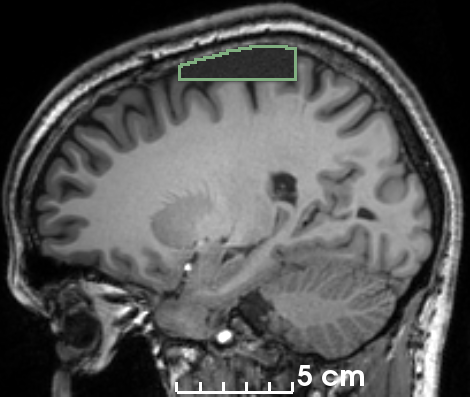
\includegraphics[width=\linewidth]{exp_shape_cuboid}
    \caption{\label{fig:exp_shape_cuboid}}
  \end{subfigure}
  \hfill
  \begin{subfigure}{0.32\textwidth}
    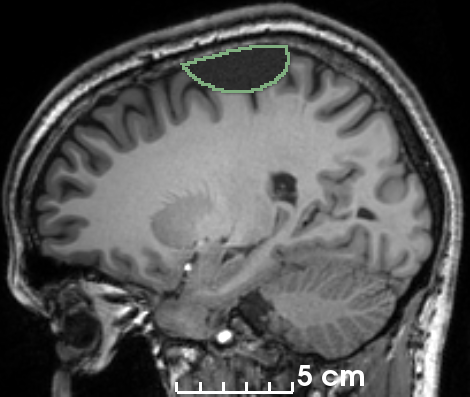
\includegraphics[width=\linewidth]{exp_shape_ellipsoid}
    \caption{\label{fig:exp_shape_ellipsoid}}
  \end{subfigure}
  \hfill
  \begin{subfigure}{0.32\textwidth}
    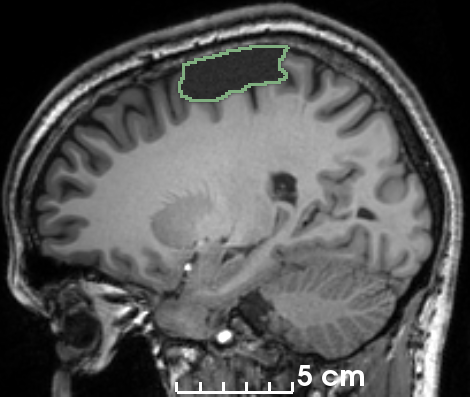
\includegraphics[width=\linewidth]{exp_shape_noisy}
    \caption{\label{fig:exp_shape_noisy}}
  \end{subfigure}

  \caption[Simulation of resection cavities with increasing complexity]{
    Simulation of \acp{RC} with increasing shape complexity (\cref{sec:simulation}):
    cuboid (\subref{fig:exp_shape_cuboid}),
    ellipsoid (\subref{fig:exp_shape_ellipsoid})
    and ellipsoid perturbed with simplex noise (\subref{fig:exp_shape_noisy}).
  }
  \label{fig:exp_shape}
\end{figure}

\subsubsection{Fine-tuning on small clinical datasets}

We assessed the generalizability of our baseline model by fine-tuning it on small datasets from four institutions that may use different surgical approaches and acquisition protocols (including contrast enhancement and anisotropic spacing in \textit{Strasbourg}) (\cref{sec:multicenter}).
Additionally, we fine-tuned the model on 20 cases from EPISURG with the lowest \ac{DSC} in \cref{sec:self}.

For each dataset, we load the pretrained baseline model, initialize the optimizer with an initial learning rate of $5 \times 10^{-4}$, initialize the learning rate scheduler and fine-tune all layers simultaneously for 40 epochs using 5-fold cross-validation.
We use model weights from the epoch with the lowest mean validation loss for evaluation.
To minimize data leakage, we determined the above hyperparameters using the validation set of one fold in the \textit{Milan} dataset.

We observed a consistent increase in \ac{DSC} for all fine-tuned models, up to a maximum of 89.2 (13.3) for the \textit{Milan} dataset.
For comparison, inter-rater agreement between human annotators in our previous study was 84.0 (9.9) \cite{perez-garcia_simulation_2020}.
Quantitative and qualitative evaluations are illustrated in \cref{fig:finetuning_quant,fig:finetuning_qual}, respectively.


\begin{figure}
  \centering
  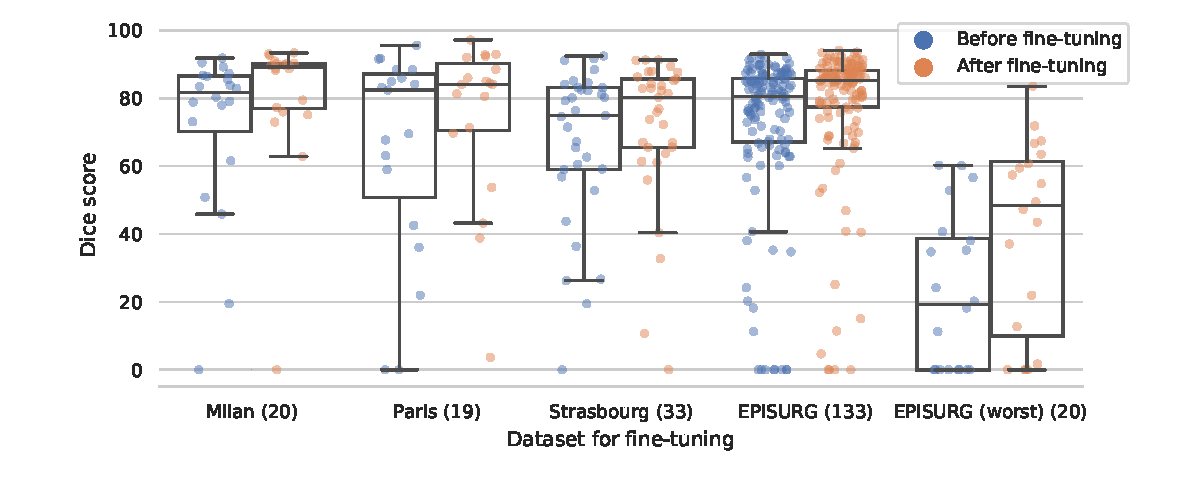
\includegraphics[trim=1cm 0 0.8cm 0, clip, width=\linewidth]{boxplot_finetuning}
  \caption[Dice score without before and after fine-tuning]{
    \ac{DSC} without (blue) and with (orange) fine-tuning of the model training using self-supervision.
    Horizontal lines in the boxes represent the first, second (median) and third quartiles.
    The `EPISURG (worst)' dataset comprises the 20 cases from EPISURG with the lowest \ac{DSC} in the experiment described in \cref{sec:self}.
    Numbers in parentheses indicate subjects per dataset.
  }
  \label{fig:finetuning_quant}
\end{figure}


\begin{figure}[ht!]
  \centering
  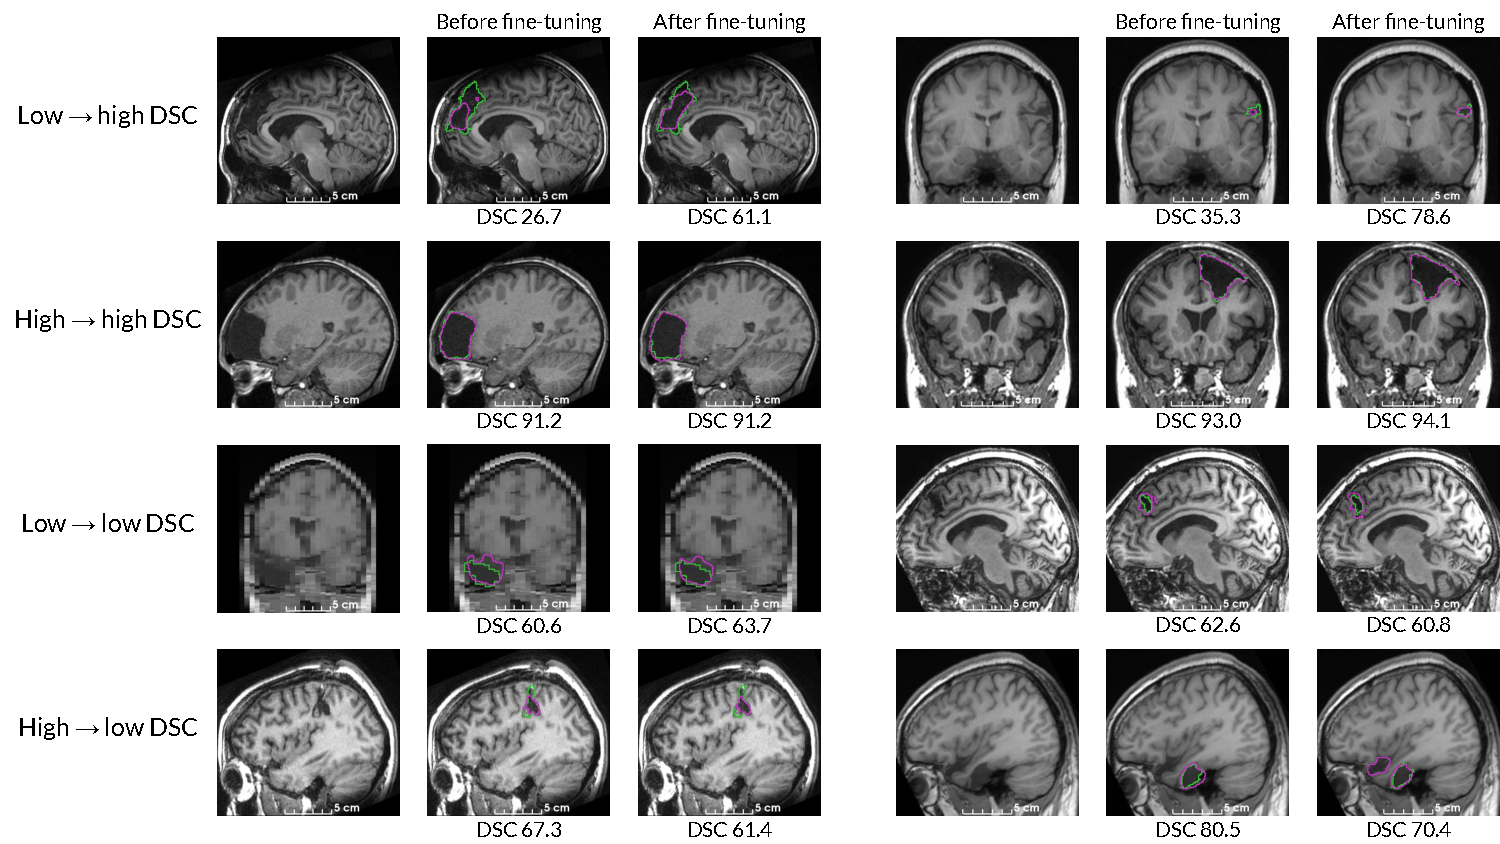
\includegraphics[width=\linewidth]{finetune}
  \caption[Qualitative evaluation of fine-tuning]{
    Qualitative evaluation of fine-tuning for the \textit{Strasbourg} (left) and EPISURG (right) datasets.
    Rows correspond, from top to bottom, to cases for which the \ac{DSC}
    1) increased,
    2) remained high,
    3) remained low and
    4) decreased
    after fine-tuning the self-supervised model.
    Manual annotations (green) and model predictions (magenta) are overlaid.
  }
  \label{fig:finetuning_qual}
\end{figure}

\subsubsection{Semi-supervised learning: leveraging real unlabeled resections}
\label{sec:results_semi}

\newcommand{\pseudo}{\st{pseudo}}

In this experiment, we assessed the ability of semi-supervised learning to improve the performance of our baseline model.
We first computed the uncertainty $u(f_{\alpha\beta}, \X\post, n\st{unc})$ for $D\unl$ (\cref{sec:leveraging_semi}), all unlabeled images in EPISURG, using the baseline model and the preprocessing and augmentation transforms (\cref{sec:preprocessing_augmentation}).
We generated pseudolabels and estimated uncertainty from $n\st{unc} = 50$ Monte Carlo \ac{TTA} iterations (\cref{sec:leveraging_semi}).
To obtain the final dataset $D\pseudo = \{ (\X_{\text{postop}_i}, \wt{\Y}_{\text{cavity}_i}) \}_{i = 1}^{n\pseudo}$, we selected pseudolabels with $u(\X_{\text{postop}_i}, \cdot) < t\st{unc} = 0.2$, resulting in $n\pseudo = 256$.

We used $D\st{pre,train}$ (\cref{sec:self}) in addition to $D\pseudo$ to train a new model $\fp{sim,semi}(\cdot)$, using the same hyperparameters as in the self-supervised setting (\cref{sec:self}).
To ensure that all batches contain real resections, we use $b - b\pseudo$ images from $D\st{pre,train}$ and $b\pseudo$ images from $D\pseudo$ to compose each mini-batch of size $b$.
We chose $b\pseudo = 2$ for our experiments, i.e., 20\,\% of the images in each mini-batch contain real resection cavities.

Semi-supervised learning improved the performance of the baseline model from 80.5 (18.7) to 81.5 (17.8) ($p = 0.474$).


\begin{figure}
  \centering

  \begin{subfigure}{0.18\linewidth}
    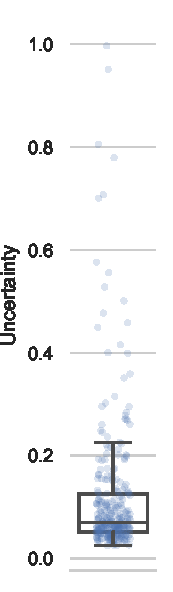
\includegraphics[width=\linewidth]{qcd}
    \caption{\label{fig:all_uncertainties}}
  \end{subfigure}
  \begin{subfigure}{0.194\linewidth}
    \begin{tabular}{c}
      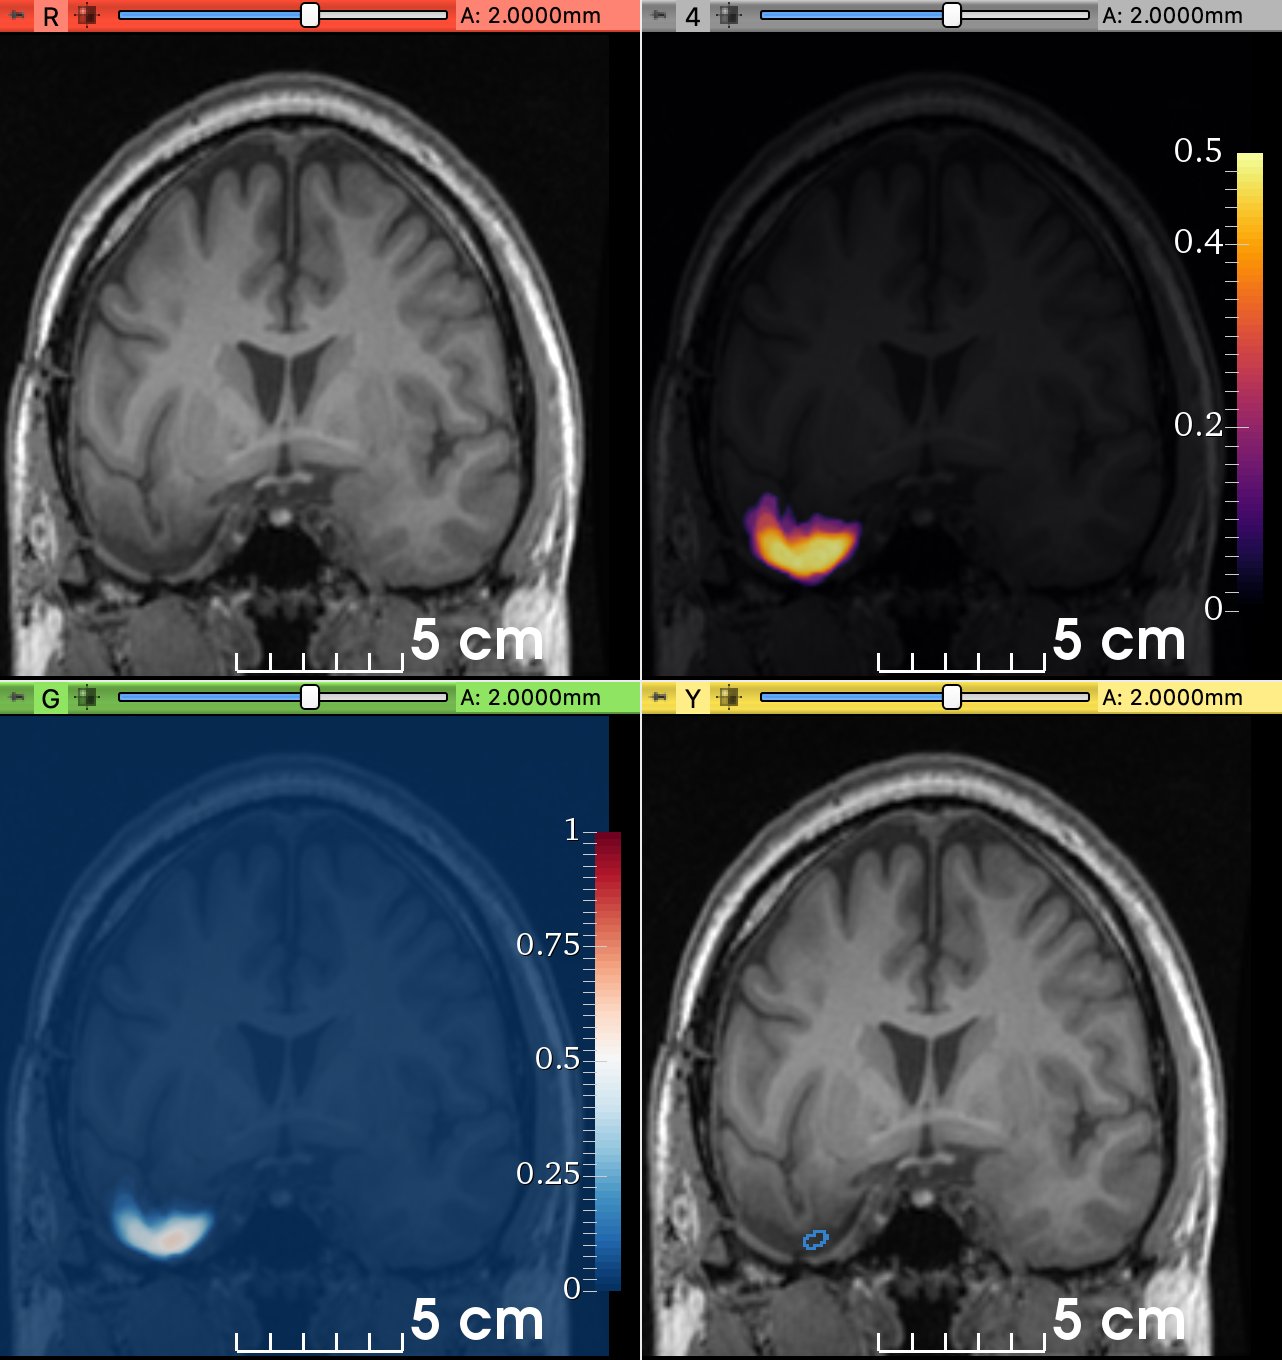
\includegraphics[trim=0 680 642 32, clip, width=\linewidth]{0796_uncertainty} \\
      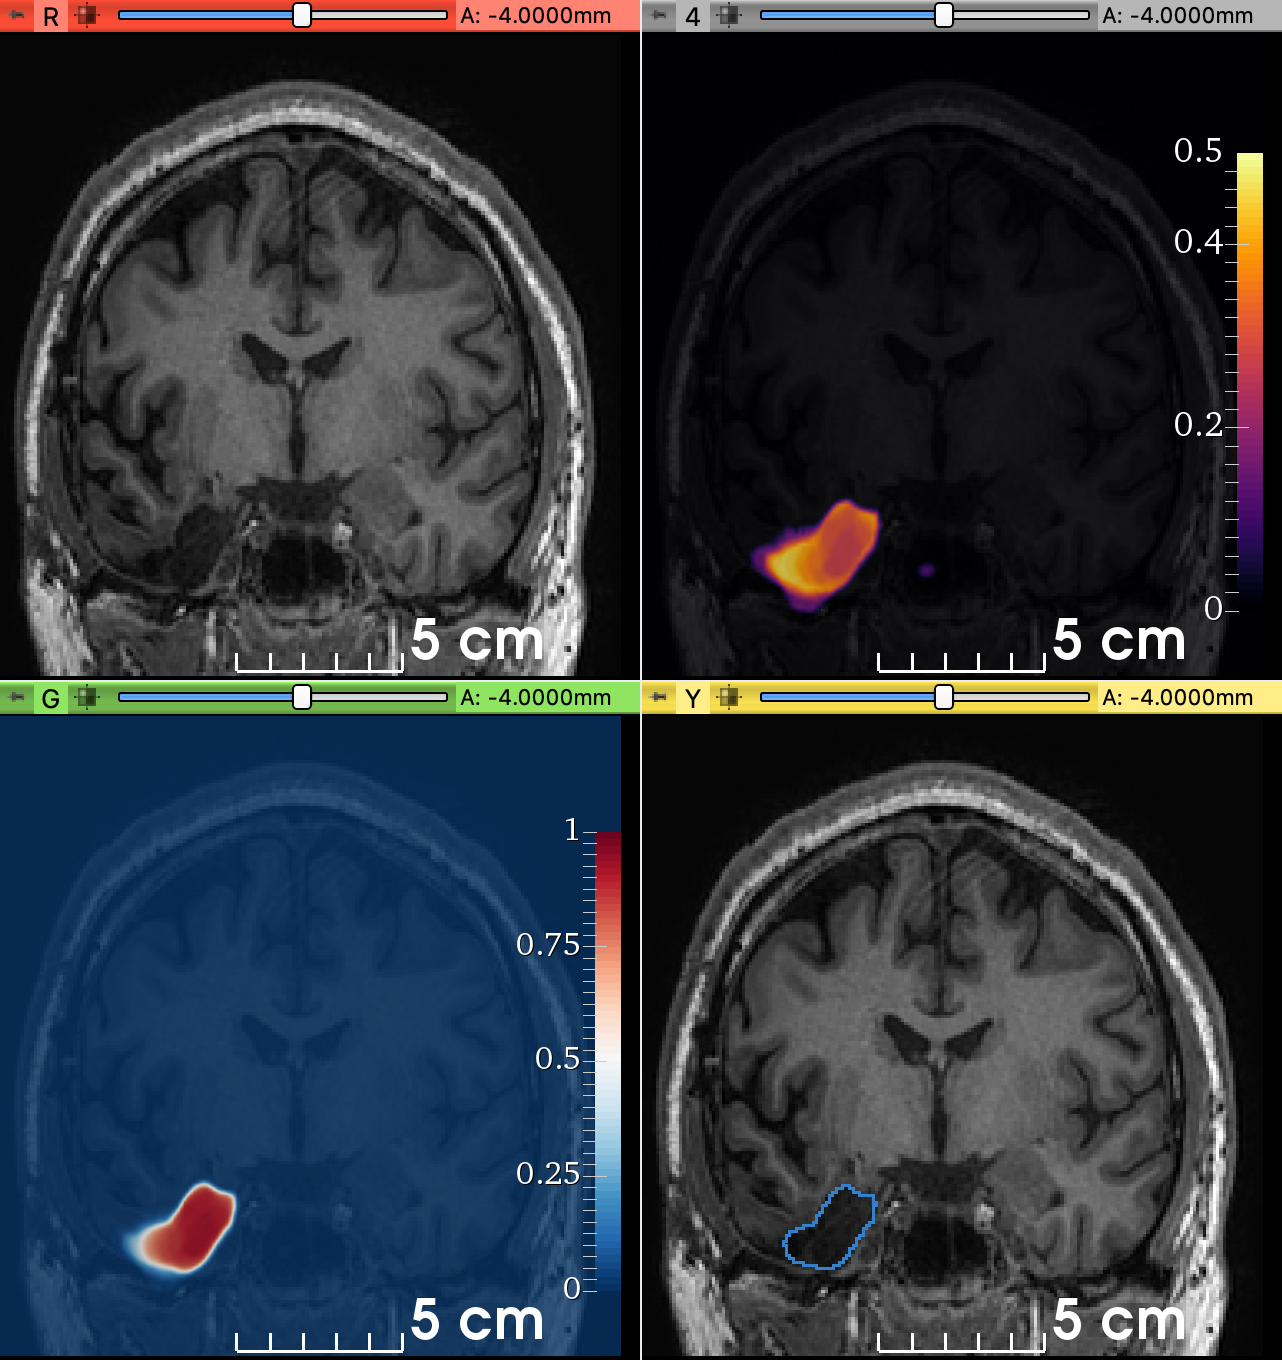
\includegraphics[trim=0 680 642 32, clip, width=\linewidth]{0914_uncertainty} \\
      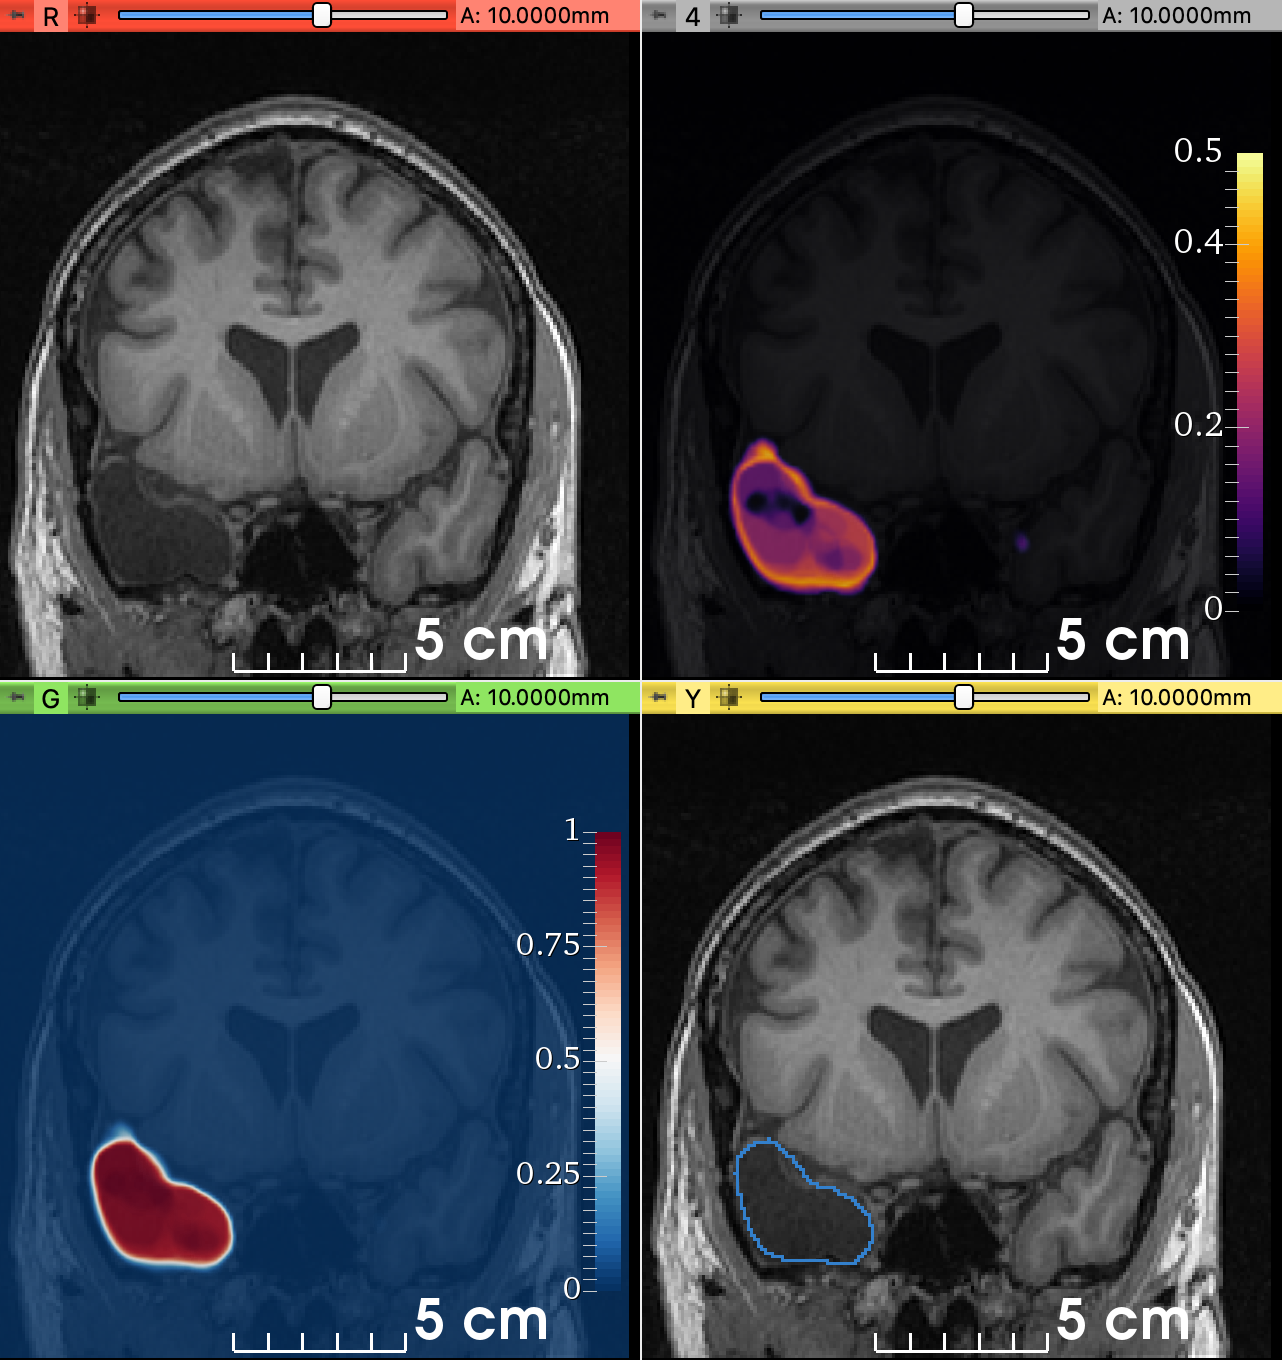
\includegraphics[trim=0 680 642 32, clip, width=\linewidth]{0499_uncertainty} \\
    \end{tabular}
    \caption{\label{fig:uncertainty_mri}}
  \end{subfigure}
  \begin{subfigure}{0.194\linewidth}
    \begin{tabular}{c}
      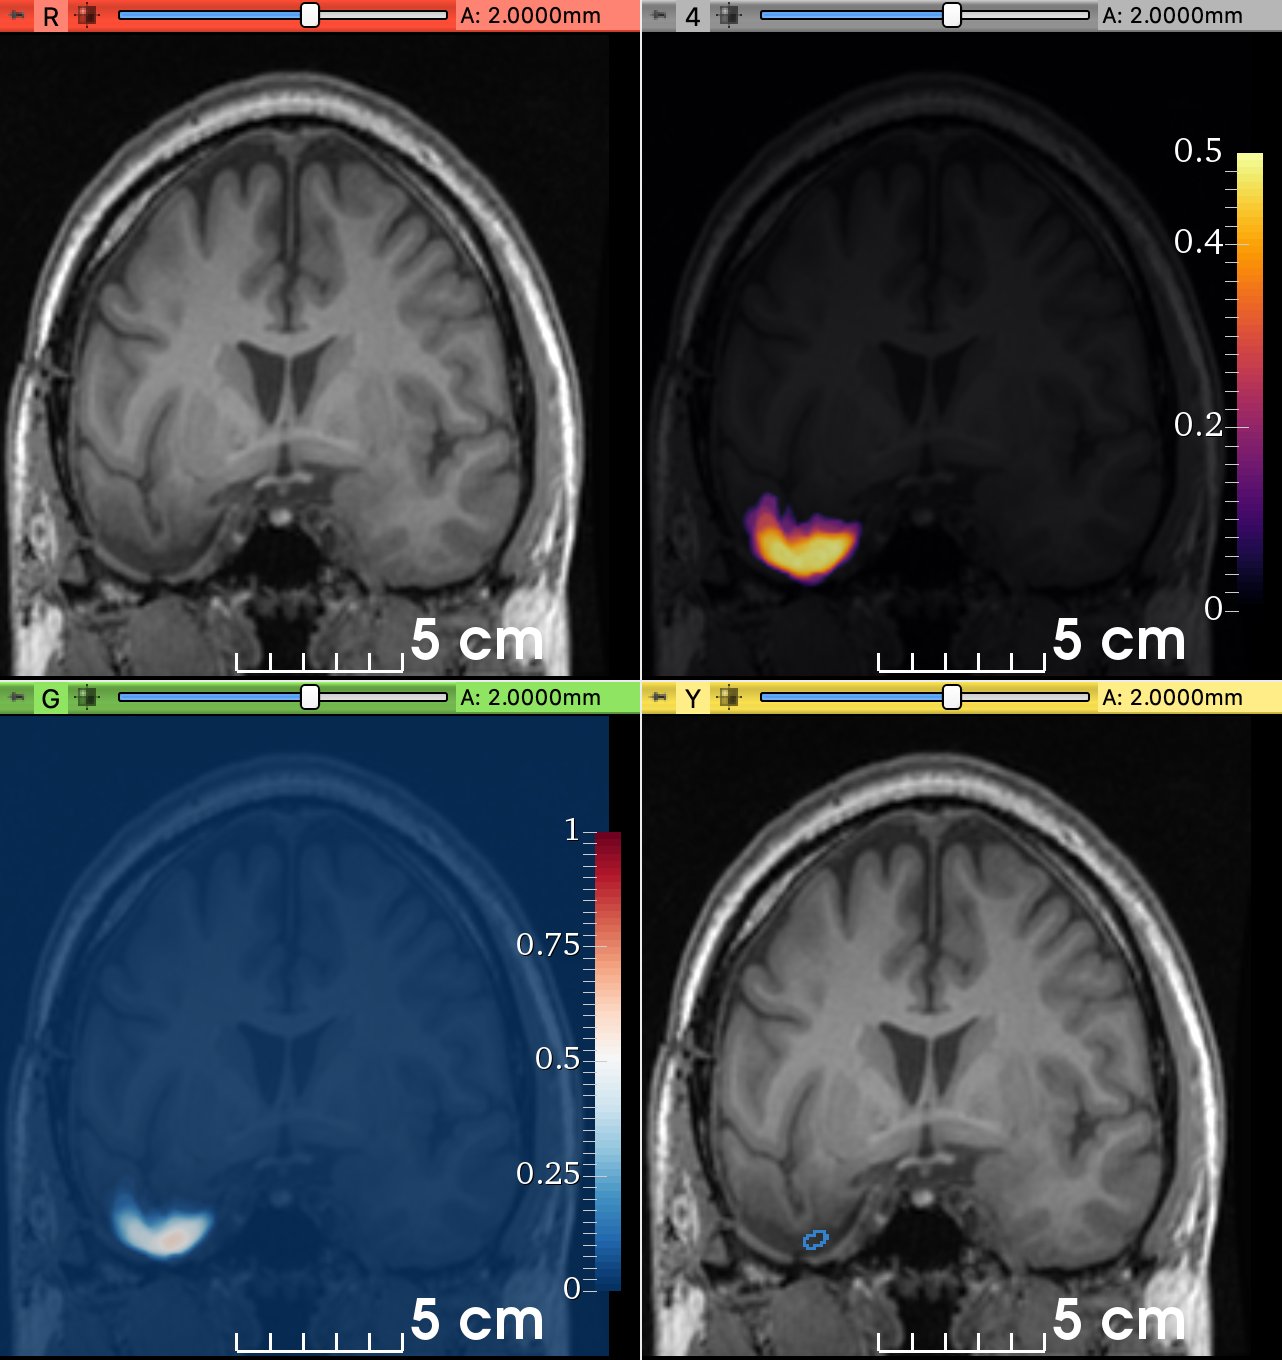
\includegraphics[trim=642 680 0 32, clip, width=\linewidth]{0796_uncertainty} \\
      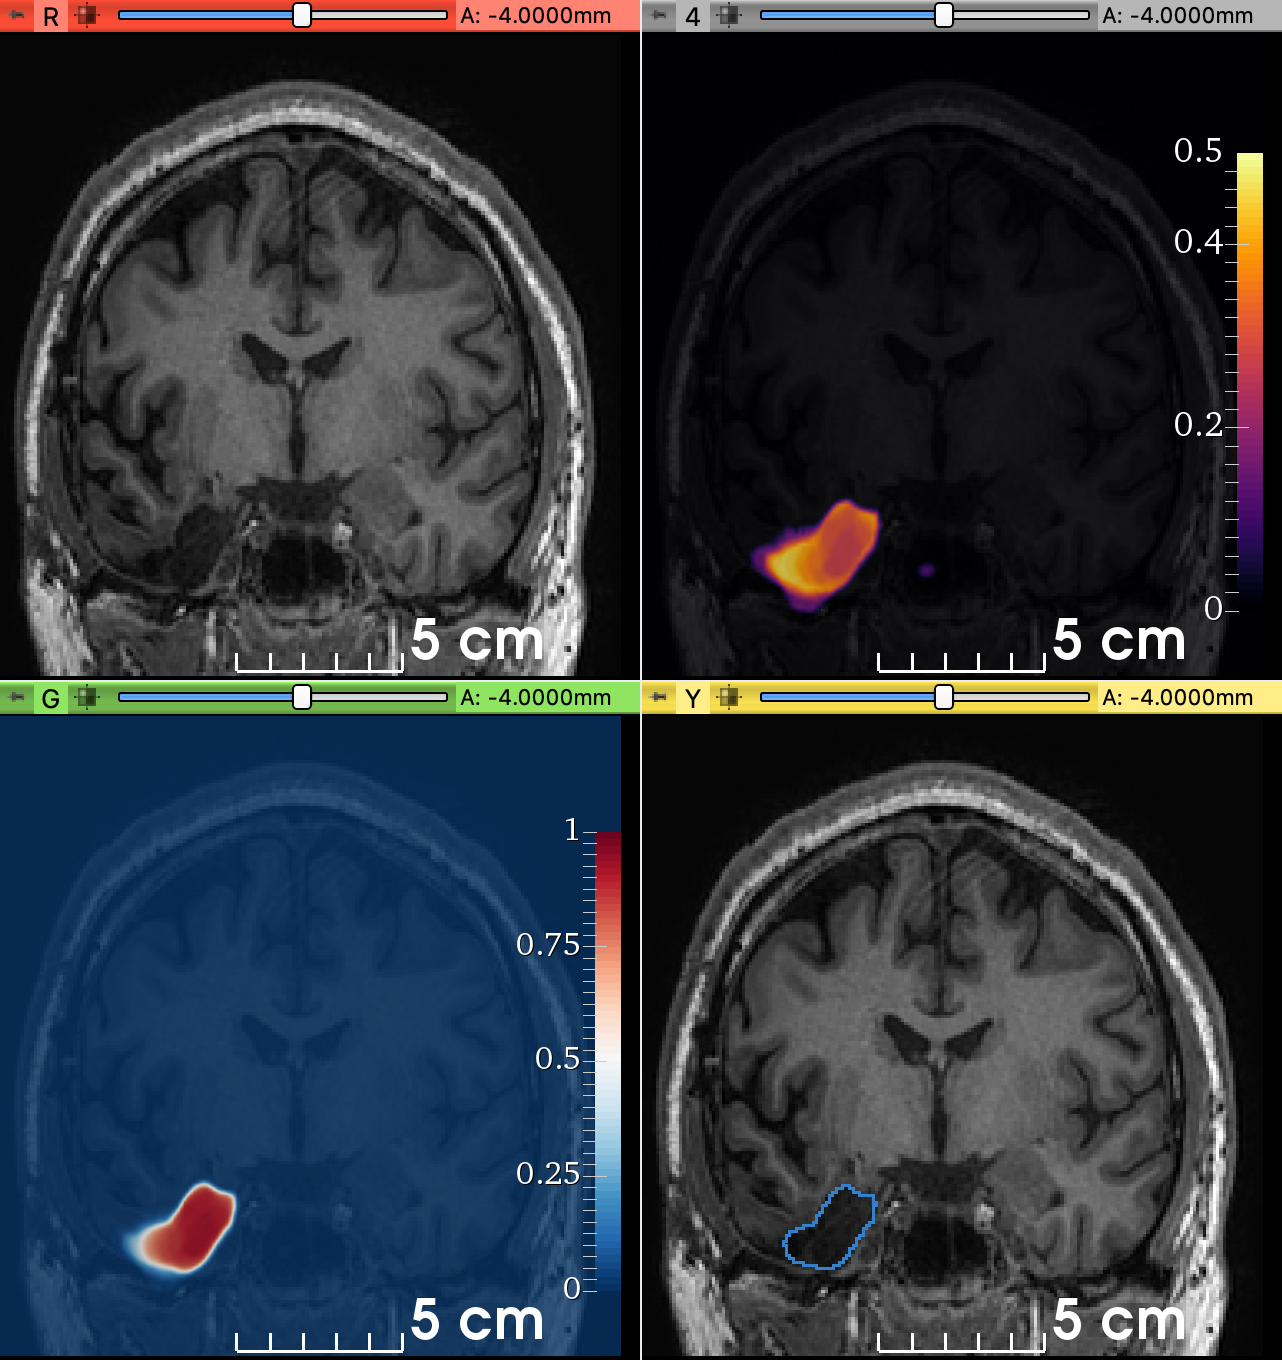
\includegraphics[trim=642 680 0 32, clip, width=\linewidth]{0914_uncertainty} \\
      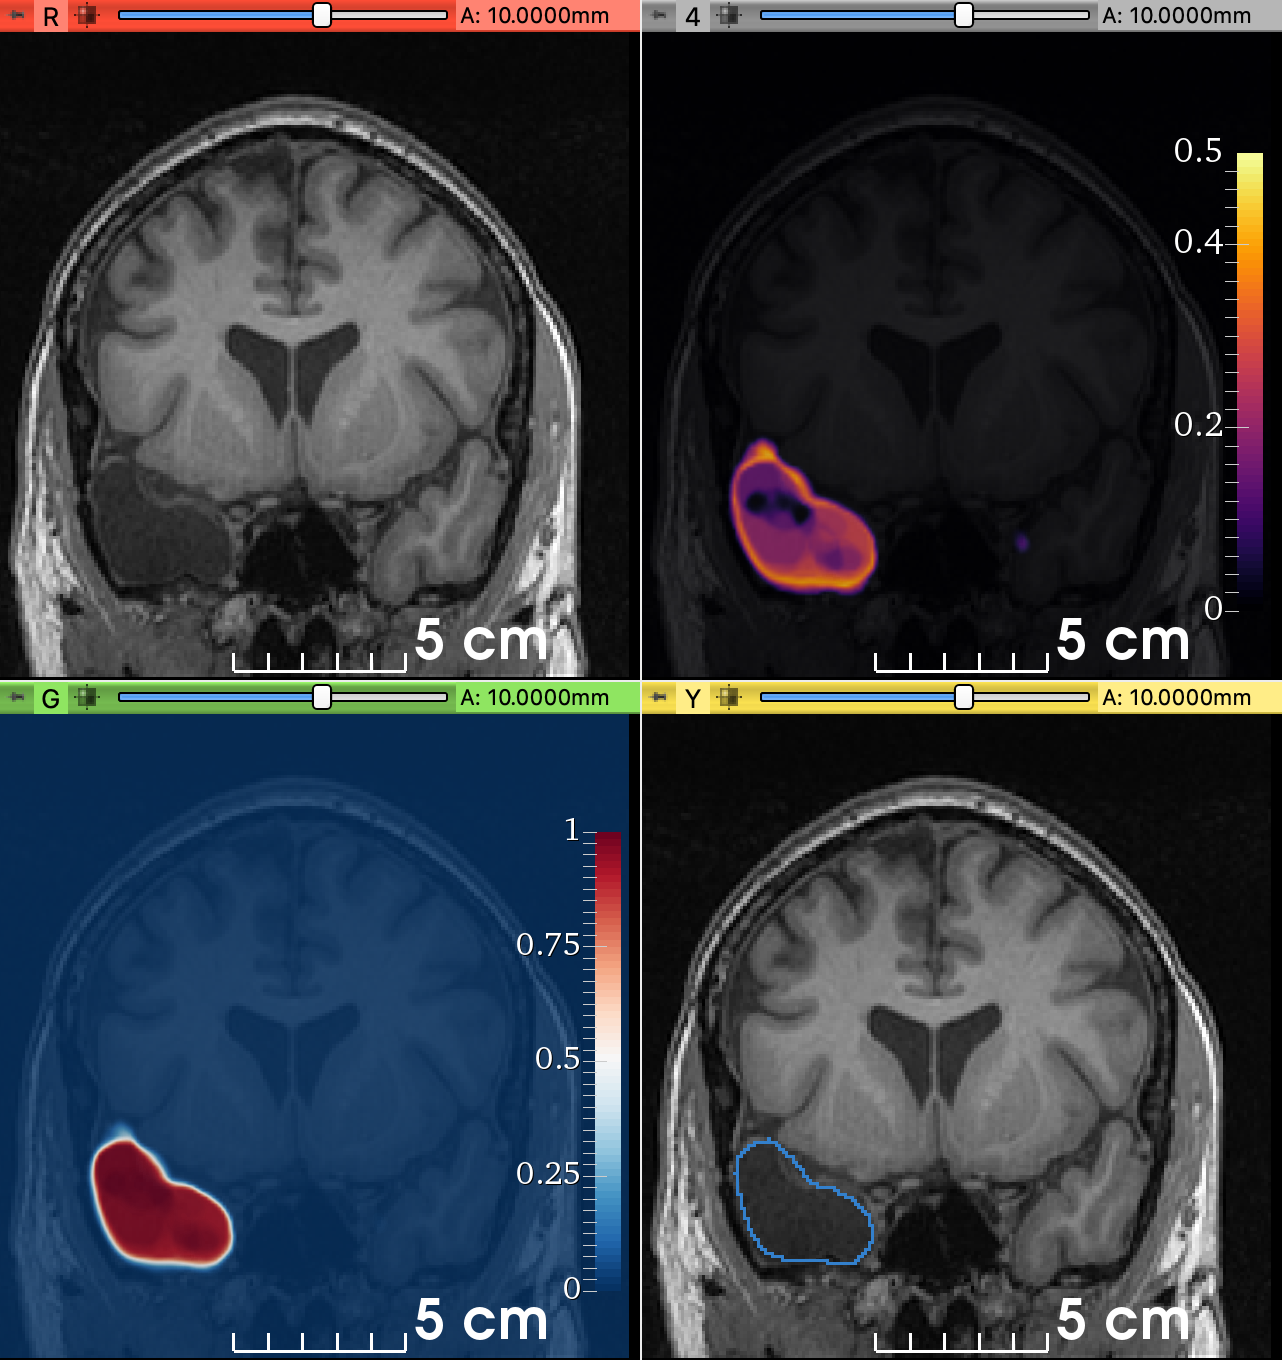
\includegraphics[trim=642 680 0 32, clip, width=\linewidth]{0499_uncertainty} \\
    \end{tabular}
    \caption{\label{fig:uncertainty_std}}
  \end{subfigure}
  \begin{subfigure}{0.194\linewidth}
    \begin{tabular}{c}
      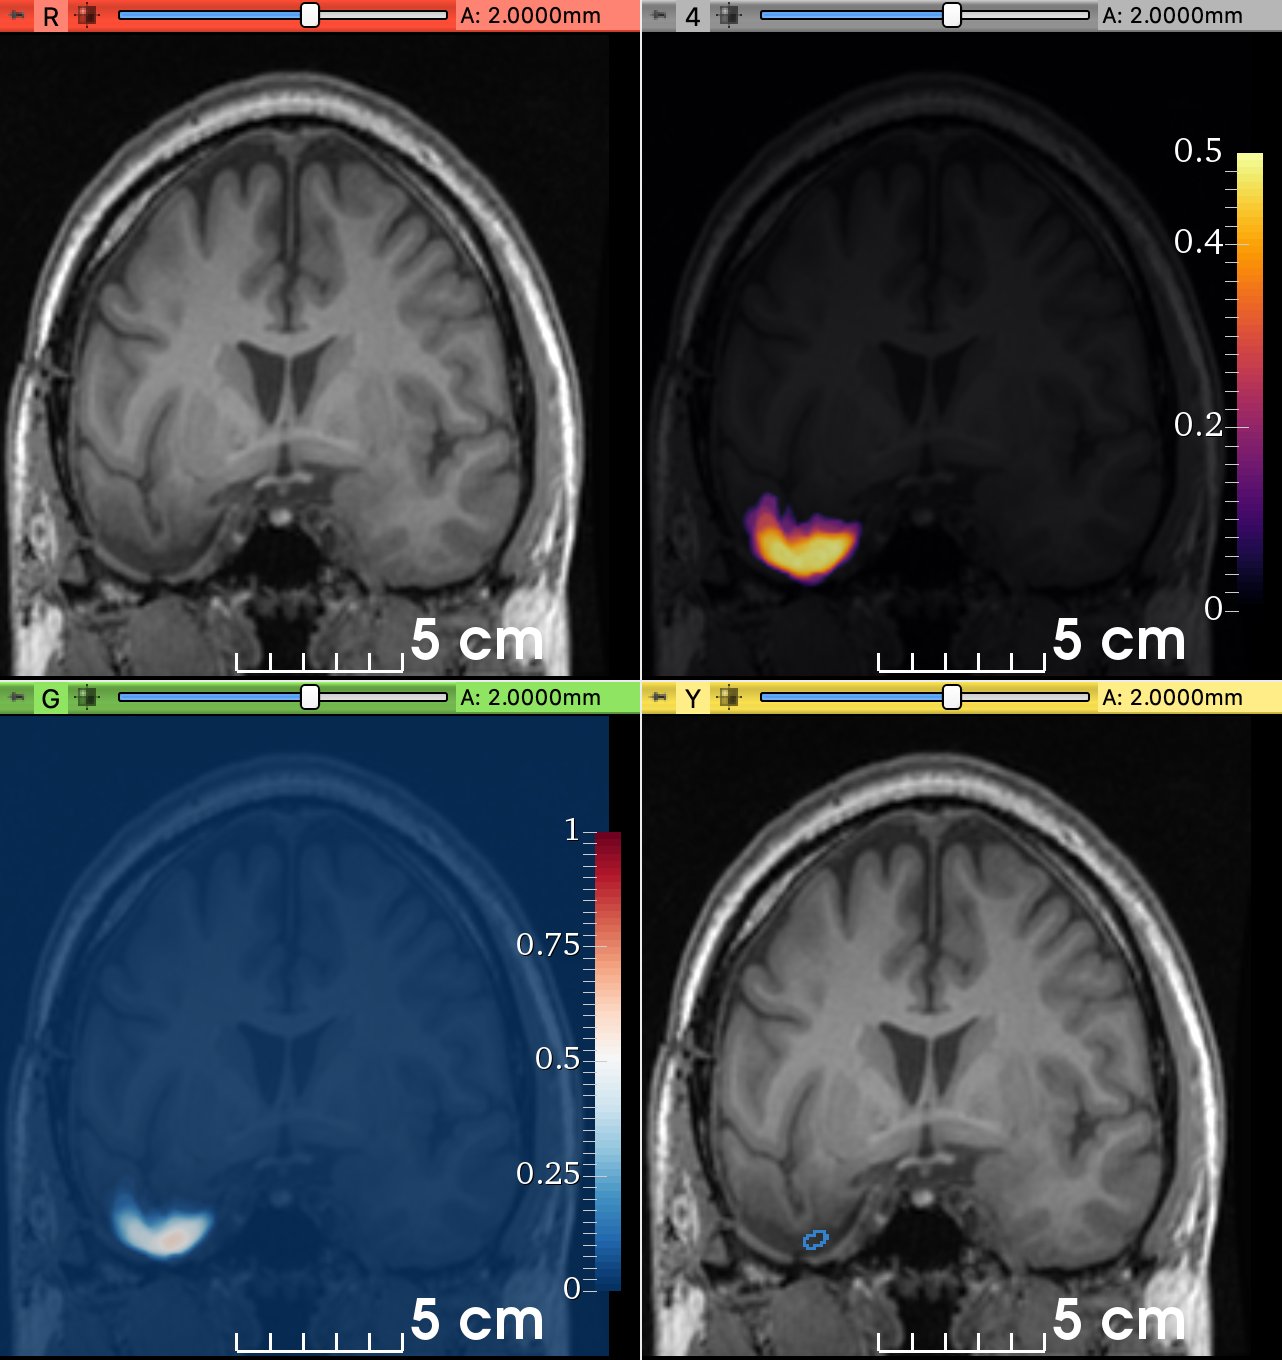
\includegraphics[trim=0 0 642 714, clip, width=\linewidth]{0796_uncertainty} \\
      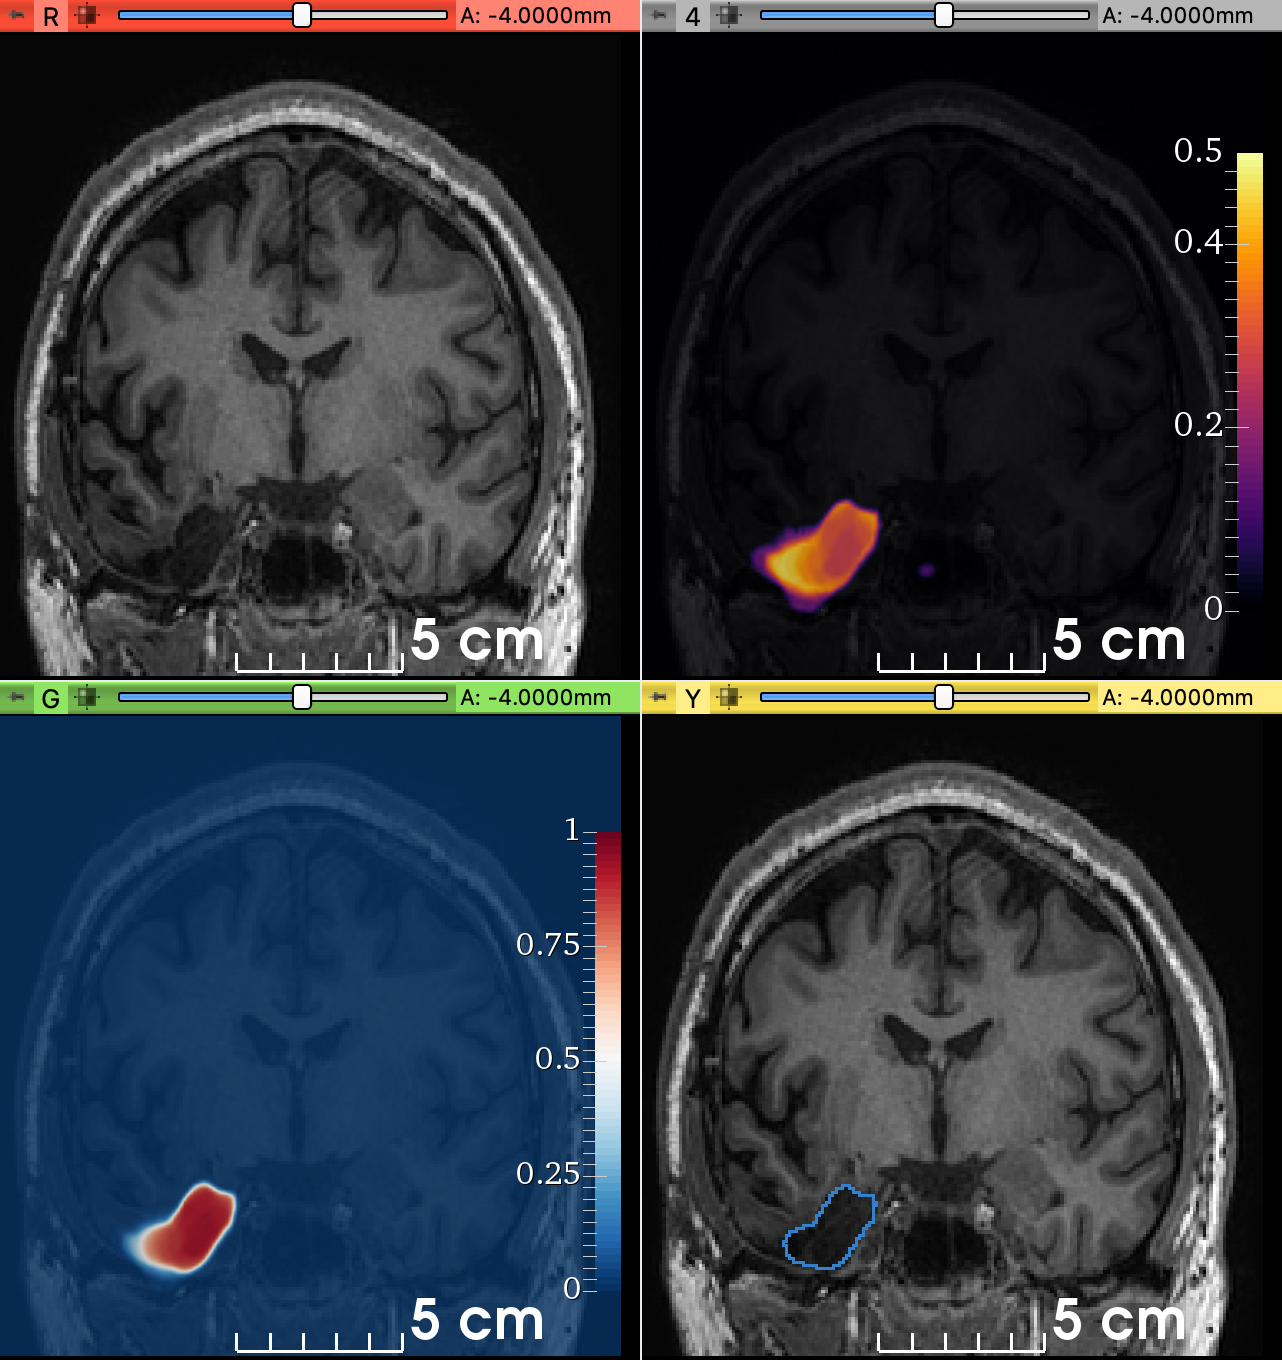
\includegraphics[trim=0 0 642 714, clip, width=\linewidth]{0914_uncertainty} \\
      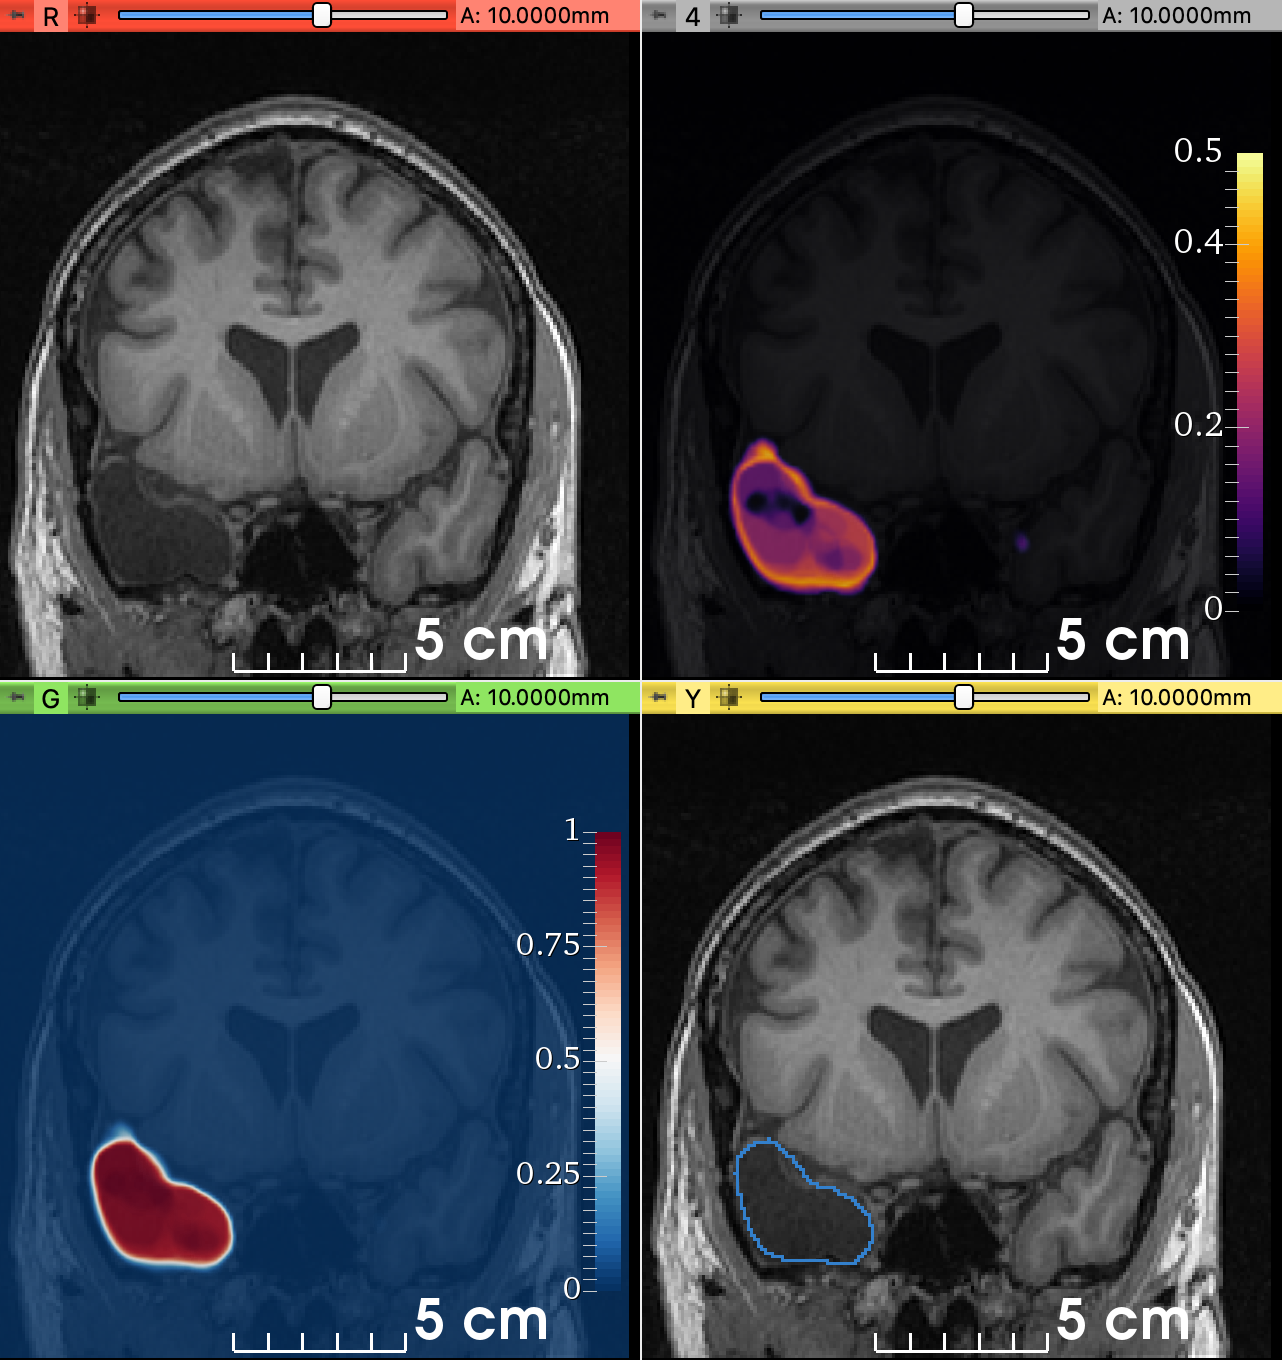
\includegraphics[trim=0 0 642 714, clip, width=\linewidth]{0499_uncertainty} \\
    \end{tabular}
    \caption{\label{fig:uncertainty_mean}}
  \end{subfigure}
  \begin{subfigure}{0.194\linewidth}
    \begin{tabular}{c}
      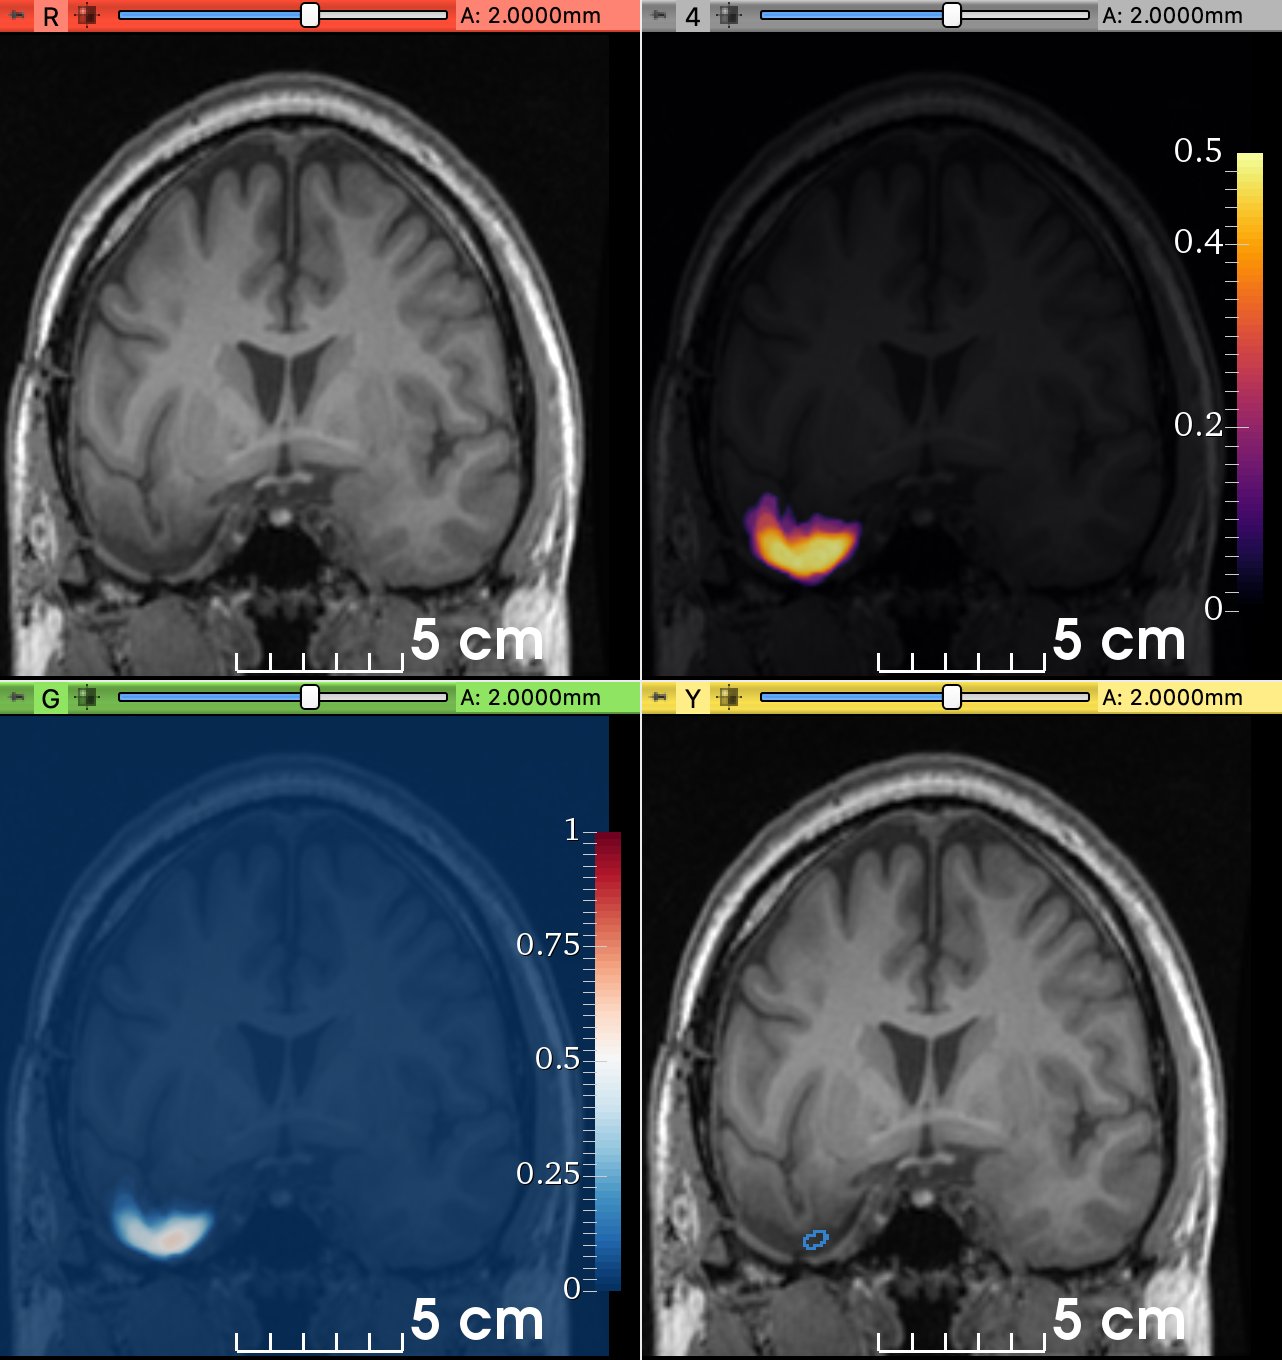
\includegraphics[trim=642 0 0 714, clip, width=\linewidth]{0796_uncertainty} \\
      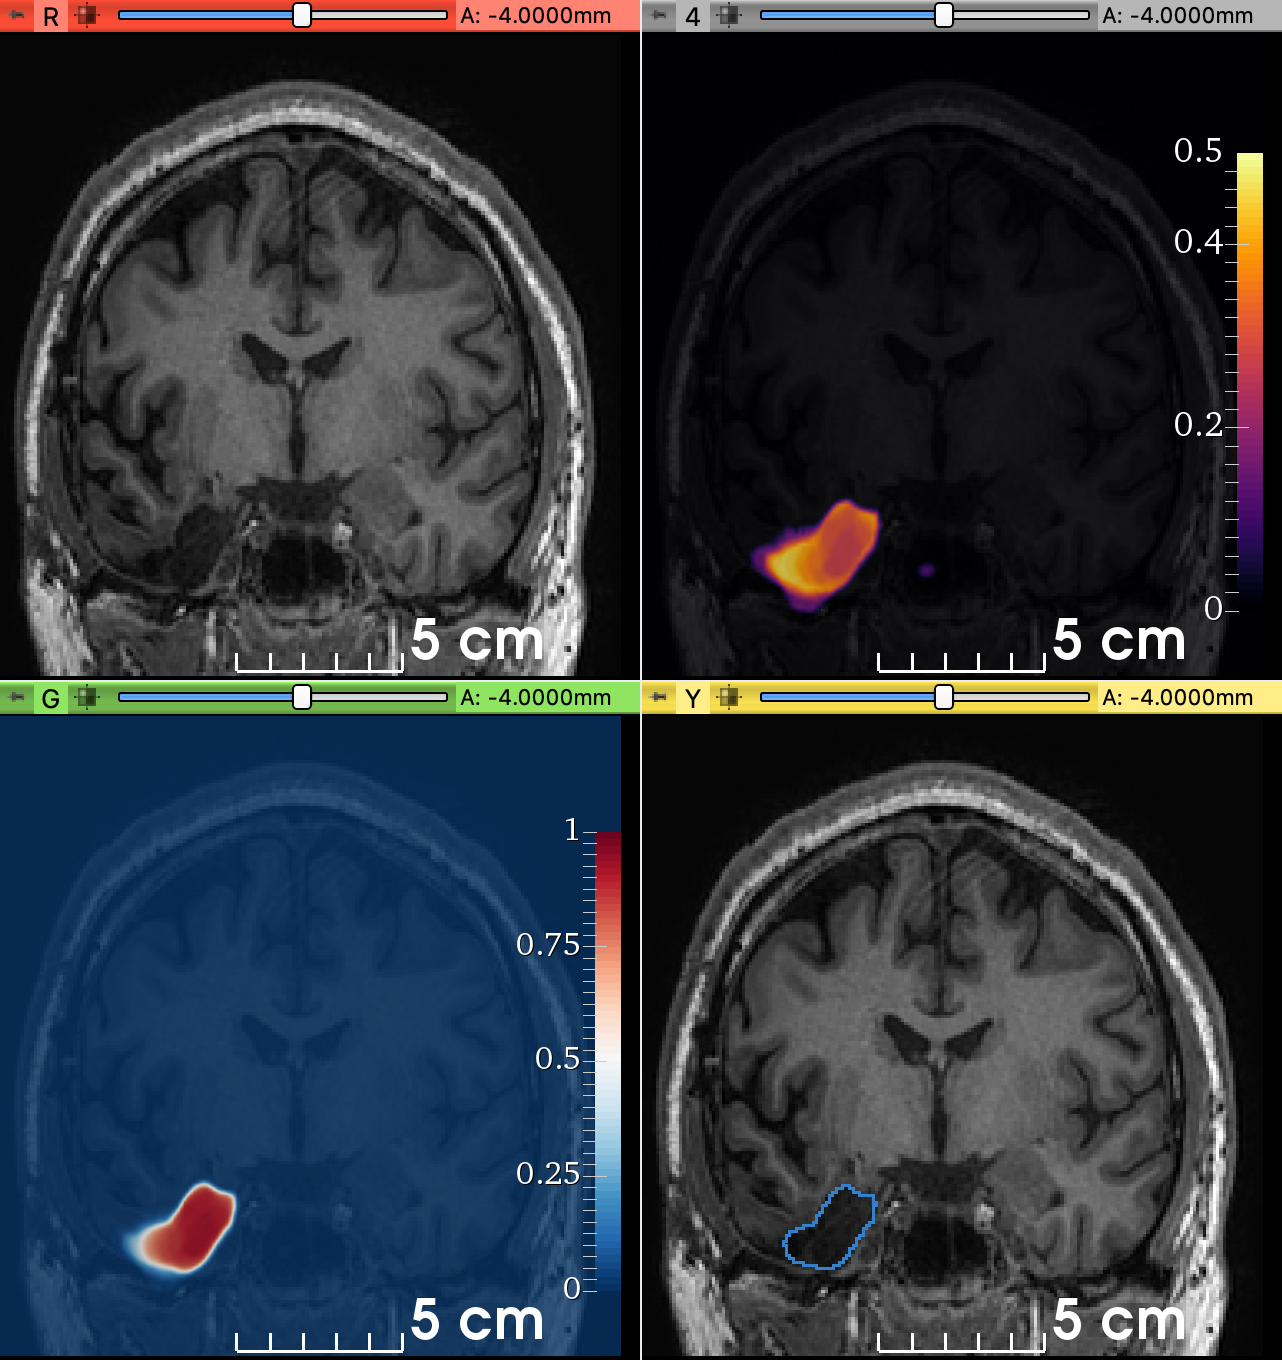
\includegraphics[trim=642 0 0 714, clip, width=\linewidth]{0914_uncertainty} \\
      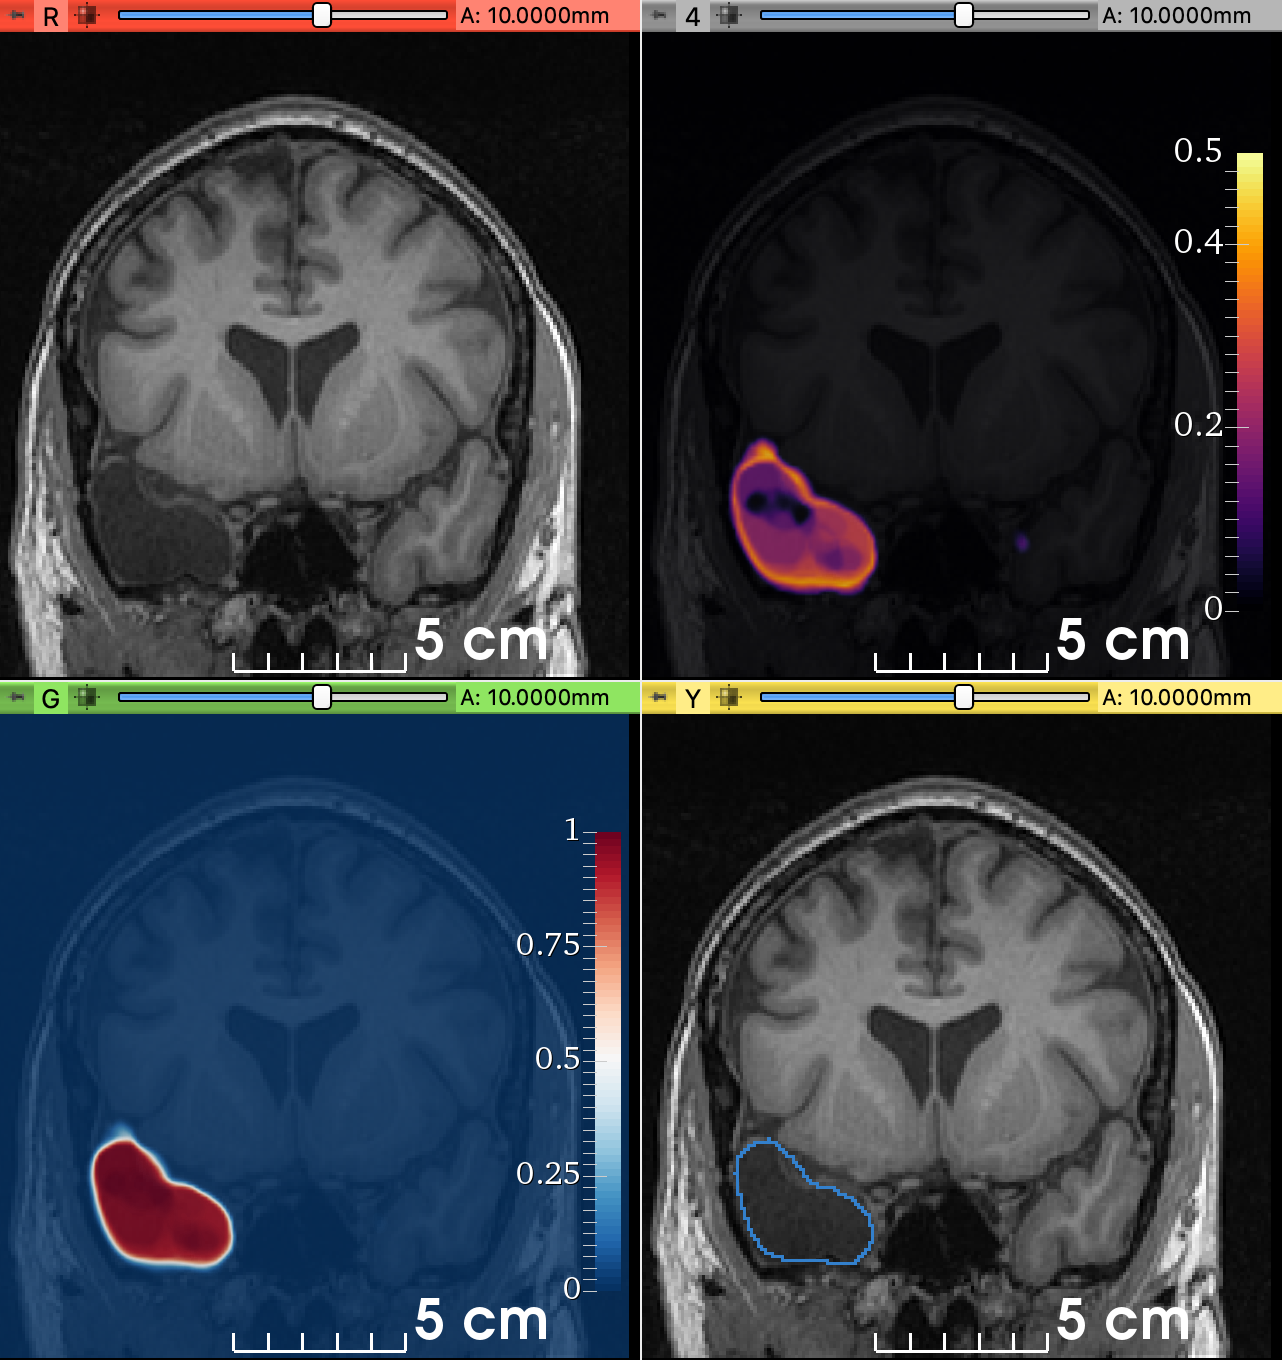
\includegraphics[trim=642 0 0 714, clip, width=\linewidth]{0499_uncertainty} \\
    \end{tabular}
    \caption{\label{fig:uncertainty_pseudo}}
  \end{subfigure}

  \caption[Generating reliable pseudolabels for semi-supervised learning]{
    Generating reliable pseudolabels for semi-supervised learning.
    Image-level uncertainty for the 297 unlabeled postoperative images in EPISURG (\subref{fig:all_uncertainties}).
    Unlabeled postoperative \acf{T1w} \ac{MRI} (\subref{fig:uncertainty_mri}).
    Voxel-wise uncertainty (\subref{fig:uncertainty_std}) estimated as the standard deviation of the probabilities across all Monte Carlo iterations.
    The mean prediction (\subref{fig:uncertainty_mean}) is thresholded at 0.5 to generate the pseudolabel (\subref{fig:uncertainty_pseudo}).
    Image-level uncertainties for the three cases are 0.805 (top), 0.195 (middle) and 0.025 (bottom).
  }
  \label{fig:uncertainties}
\end{figure}

\subsubsection{Qualitative evaluation on brain tumor resection dataset}

We used the \ac{BITE} dataset \cite{mercier_online_2012} to evaluate the ability of our self-supervised model to segment resection cavities on images from a different institution, modality and pathology than the datasets used for quantitative evaluation.
For postprocessing, all but the largest binary connected component were removed.
The model successfully segmented the resection cavity on 11/13 images, even though some contained challenging features (\cref{fig:bite}).

\newcommand{\qualit}[1]{\includegraphics[width=0.14\linewidth]{bite/cropped/#1}}
\newcommand{\qualitfig}[1]{
  \centering
  \qualit{#1_sag}%
  \enskip
  \qualit{#1_seg_sag}%
  \quad
  \qualit{#1_cor}%
  \enskip
  \qualit{#1_seg_cor}%
  \quad
  \qualit{#1_axi}%
  \enskip
  \qualit{#1_seg_axi}
}

% https://tex.stackexchange.com/a/381477/216202
\begin{figure}
  \centering
  \begin{subfigure}{\textwidth}
    \qualitfig{2_low_contrast}
    \caption{Image with low contrast between the cavity and the brain \label{fig:bite_low_contrast}}
  \end{subfigure}
  \vskip\baselineskip
  \begin{subfigure}{\textwidth}
    \qualitfig{4_air}
    \caption{Image with air and CSF within the cavity \label{fig:bite_air}}
  \end{subfigure}
  \vskip\baselineskip
  \begin{subfigure}{\textwidth}
    \qualitfig{5_aniso}
    \caption{Image with a highly anisotropic voxel spacing \label{fig:bite_aniso}}
  \end{subfigure}
  \vskip\baselineskip
  \begin{subfigure}{\textwidth}
    \qualitfig{12_motion}
    \caption{Image with \ac{MRI} motion artifacts and adjacent edema \label{fig:bite_motion}}
  \end{subfigure}
  \caption[Qualitative evaluation on postoperative brain tumor data]{
    Qualitative evaluation of the self-supervised model on a dataset of postoperative brain tumor \ac{T1wCE} \ac{MRI}.
    The model is robust to multiple challenging scenarios:
    low contrast between the cavity and the brain (\subref{fig:bite_low_contrast}),
    air and \ac{CSF} within the resection cavity (\subref{fig:bite_air}),
    highly anisotropic voxel spacing (\subref{fig:bite_aniso}),
    motion artifacts and edema (\subref{fig:bite_motion}),
    and a different modality than used for training (all).
    Note that these images are from a different institution, modality and pathology than the datasets used for quantitative evaluation.
    Ground-truth labels are not shown as manual annotations are not available.
  }
  \label{fig:bite}
\end{figure}




\subsubsection{Qualitative evaluation on intraoperative image}

We used our baseline model to segment the resection cavity on one intraoperative \ac{MRI} from our institution.
Despite the large domain shift between the training dataset and the intraoperative image, which includes a retracted skin flap and a missing bone flap, the model was able to correctly estimate the resection cavity, discarding similar regions filled with \ac{CSF} or air (\cref{fig:intra}).

\begin{figure}
  \centering
  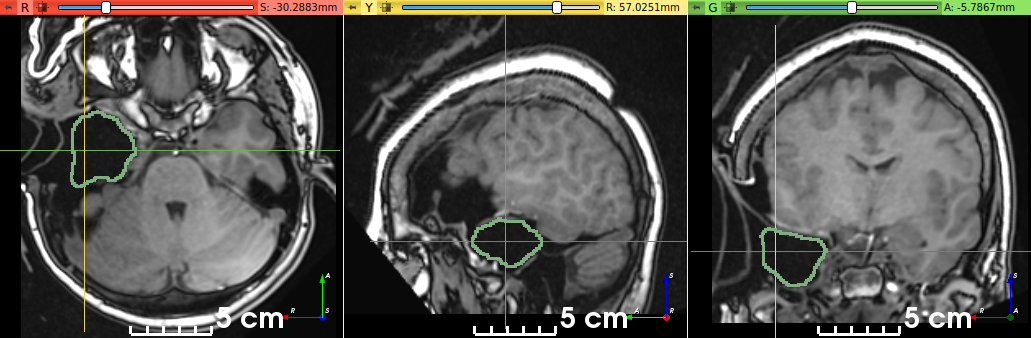
\includegraphics[trim=0 0 0 12, clip, width=\linewidth]{intra}
  \caption[Qualitative result on an intraoperative \acs{MRI}]{
    Qualitative result on an intraoperative \ac{MRI}.
    The baseline model correctly discarded regions filled with air or \ac{CSF} outside of the resection cavity.
  }
  \label{fig:intra}
\end{figure}


\section{Discussion}
\label{sec:resections_discussion}

We addressed the challenge of segmenting postoperative brain \acp{RC} from \ac{T1w} \ac{MRI} without annotated data.
We developed a self-supervised learning strategy to train without manually annotated data, and a method to simulate \acp{RC} from preoperative \ac{MRI} to generate training data.
Our novel approach is conceptually simple, easy to implement, and relies on clinical knowledge about postoperative phenomena.
The resection simulation is computationally efficient ($< \SI{1}{\second}$), so it can run during training as part of a data augmentation pipeline.
It is compatible with the TorchIO framework \cite{perez-garcia_torchio_2021} (\cref{chap:torchio}) to leverage other data argumentation techniques during training, enabling our model to have a robust performance across \ac{MRI} of variable quality.

Modeling a realistic cavity shape is important (\cref{sec:self}).
Our model generalizes well to clinical data from different institutions and pathologies, including epilepsy and glioma.
Models may be easily fine-tuned using small annotated clinical datasets to improve performance.
Moreover, our resection simulation and learning strategy may be extended to train with arbitrary modalities, or synthetic modalities generated from brain parcellations \cite{billot_learning_2020}.
Therefore, our strategy can be adopted by institutions with a large amount of unlabeled data, while fine-tuning and testing on a smaller labeled dataset.

Poor segmentation performance is often due to very small cavities, where the cavity was not detected, and large brain shift or subdural edema, where regions were incorrectly segmented.
The former issue may be overcome by training with a distribution of cavity volumes which oversamples small resections.
The latter can be addressed by extending our method to simulate displacement with biomechanical models or nonlinear deformations of the brain \cite{granados_generative_2021}.

The baseline model performance improved by leveraging unlabeled postoperative images for semi-supervised learning, but remained lower than inter-rater variability \cite{perez-garcia_simulation_2020}.  % TODO: add this info in this thesis!
We believe that a setting with a smaller training dataset might benefit further from the semi-supervised approach.
However, we did not perform an extensive assessment of our semi-supervised approach as this is out of the scope of this paper.

We showed that our model correctly segmented an intraoperative image, respecting imaginary boundaries between brain and skull, suggesting a good inductive bias of human neuroanatomy.
Qualitative results and execution time, which is in the order of milliseconds, suggest that our method could be used intraoperatively, for image guidance during resection or to improve registration with preoperative images by masking the cost function using the \ac{RC} segmentation \cite{brett_spatial_2001}.
Segmenting the \ac{RC} may also be used to study potential damage to white matter tracts postoperatively \cite{winston_optic_2012}.
Our method could be easily adapted to simulate other lesions for self-supervised training, such as cerebral microbleeds \cite{cuadrado-godia_cerebral_2018}, narrow and snake-shaped \acp{RC} typical of disconnective surgeries \cite{mohamed_temporoparietooccipital_2011}, or \acp{RC} with residual tumor \cite{meier_automatic_2017}.

As part of this work, we curated and released EPISURG, an \ac{MRI} dataset with annotations from three independent raters.
EPISURG could serve as a benchmark dataset for quantitative analysis of pre- and postoperative imaging of open resection for epilepsy treatment.
To the best of our knowledge, this is the first open annotated database of post-resection \ac{MRI} for epilepsy patients.


\onehalfspacing % a blank line seems to be needed before this command

% TODO: add stuff from MICCAI? inter-rater variability, training with smaller datasets etc
